\chapter{Materials and Methods}
\label{chap:2_materials_methods}
This chapter is devoted to describe the developed system. The development strategy was based in splitting up the functionality into different modules, which have been tackled sequentially. The next sections will cover each one of the modules, and will describe the achieved solution. Finally, the full ensemble will be described and tested.


\section{Available materials}
\label{sec:2_materials}
\subsection{Hardware}
\subsubsection{Base board}
As it was depicted in \autoref{sec:1_sota}, typical following behaviors work on a personal computer attached to a robot. However, our solution is developed using a devoted SoM: the NVIDIA Jetson TX2, similar to the one described on \autoref{fig:1_tx2}. This system features a high-performance GPU, and low-level optimization engines, which greatly reduce the time required to perform the operations required for deep learning applications, such as tensor convolutions. The low power consumption of this board (15W at full power makes it suitable to be embedded in a portable robot equipped with a battery). One drawback of this system is the scarce storage space. However, this can be immediately solved installing an external storage device using its integrated SATA connector. In this project, a 120 GB Kingston SSD (\textit{Solid State Drive}) was used for this purpose, leveraging as well on the high transference throughput this device can achieve. It features a 64-bit ARM processor, and it mounts a fully functional Linux system. As it is equipped with two WiFi antennas, a remote control interface can be easily set using SSH connections. Regarding the available RAM in the board, it is limited to 8 GB, to be shared by the GPU and the CPU. This jeopardizes the execution of the deployed software and the neural networks, which have to be controlled in every moment in order to save the maximum amount of RAM possible. The resulting board can be visualized on \autoref{fig:2_mytx2}.\\

\begin{figure}[h]
	\begin{subfigure}[h]{0.45\linewidth}
		\centering
		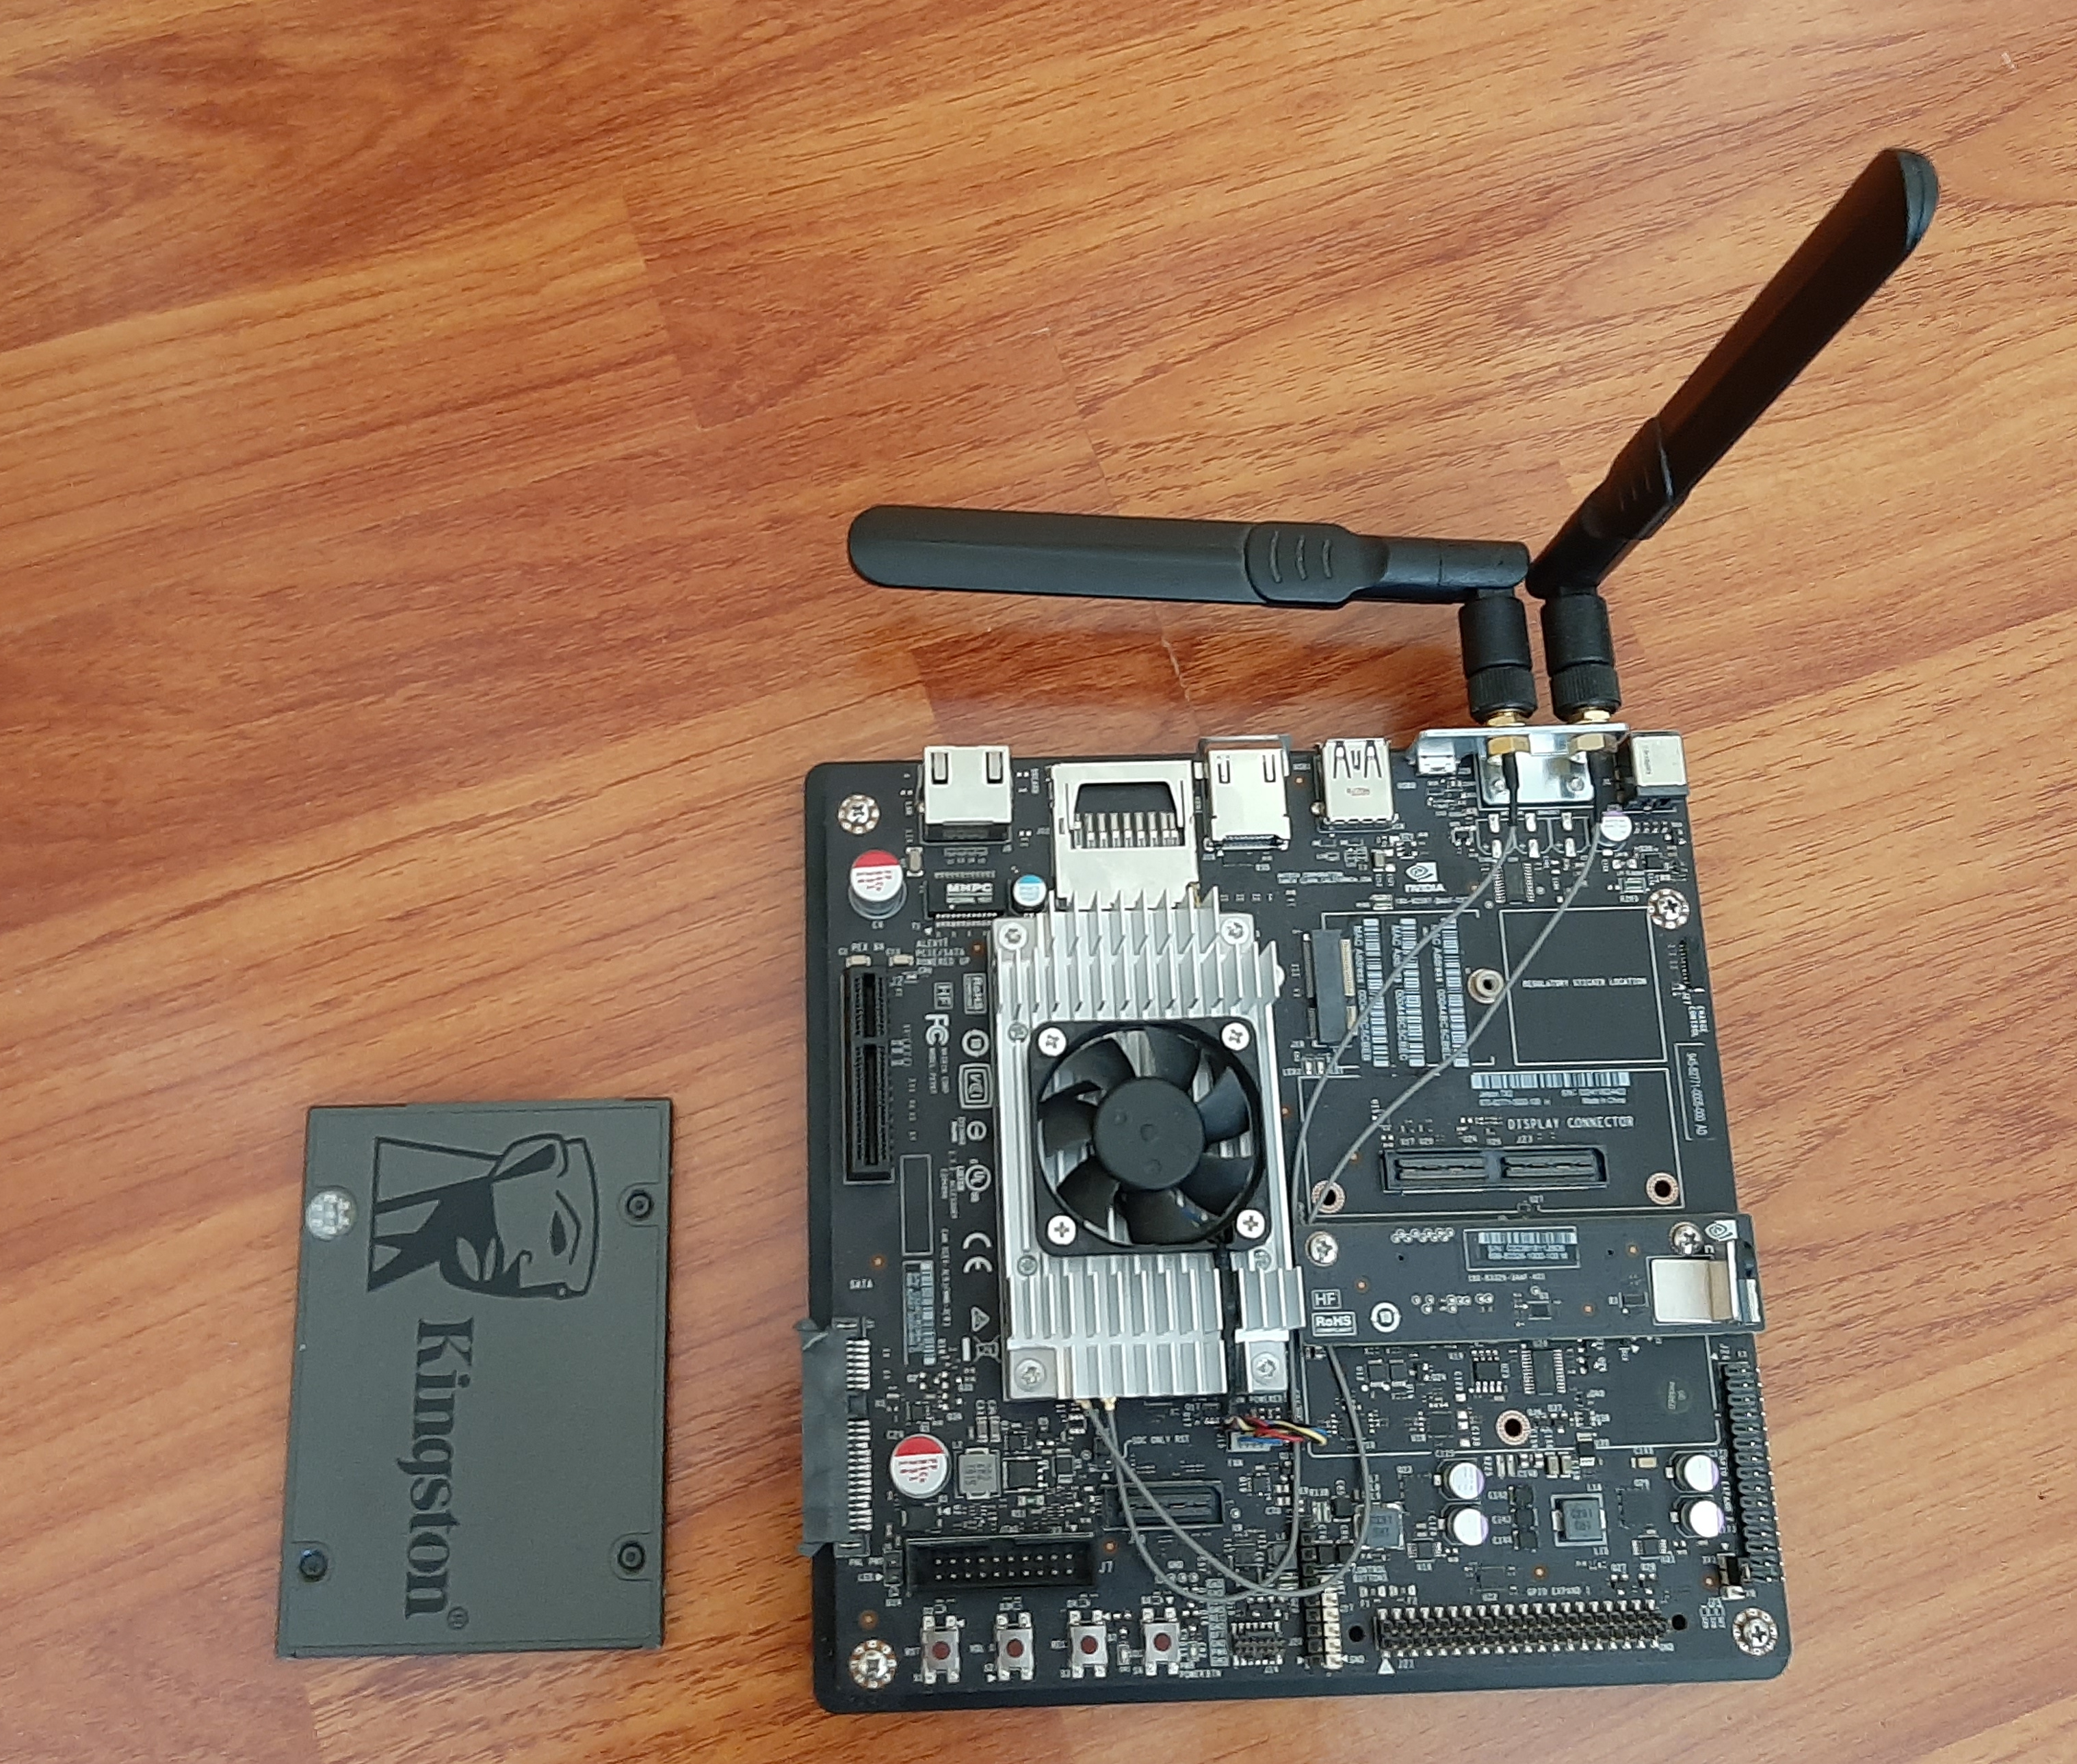
\includegraphics[width=0.98\linewidth]{tx2_nossd}
	\end{subfigure}
	\begin{subfigure}[h]{0.45\linewidth}
		\centering
		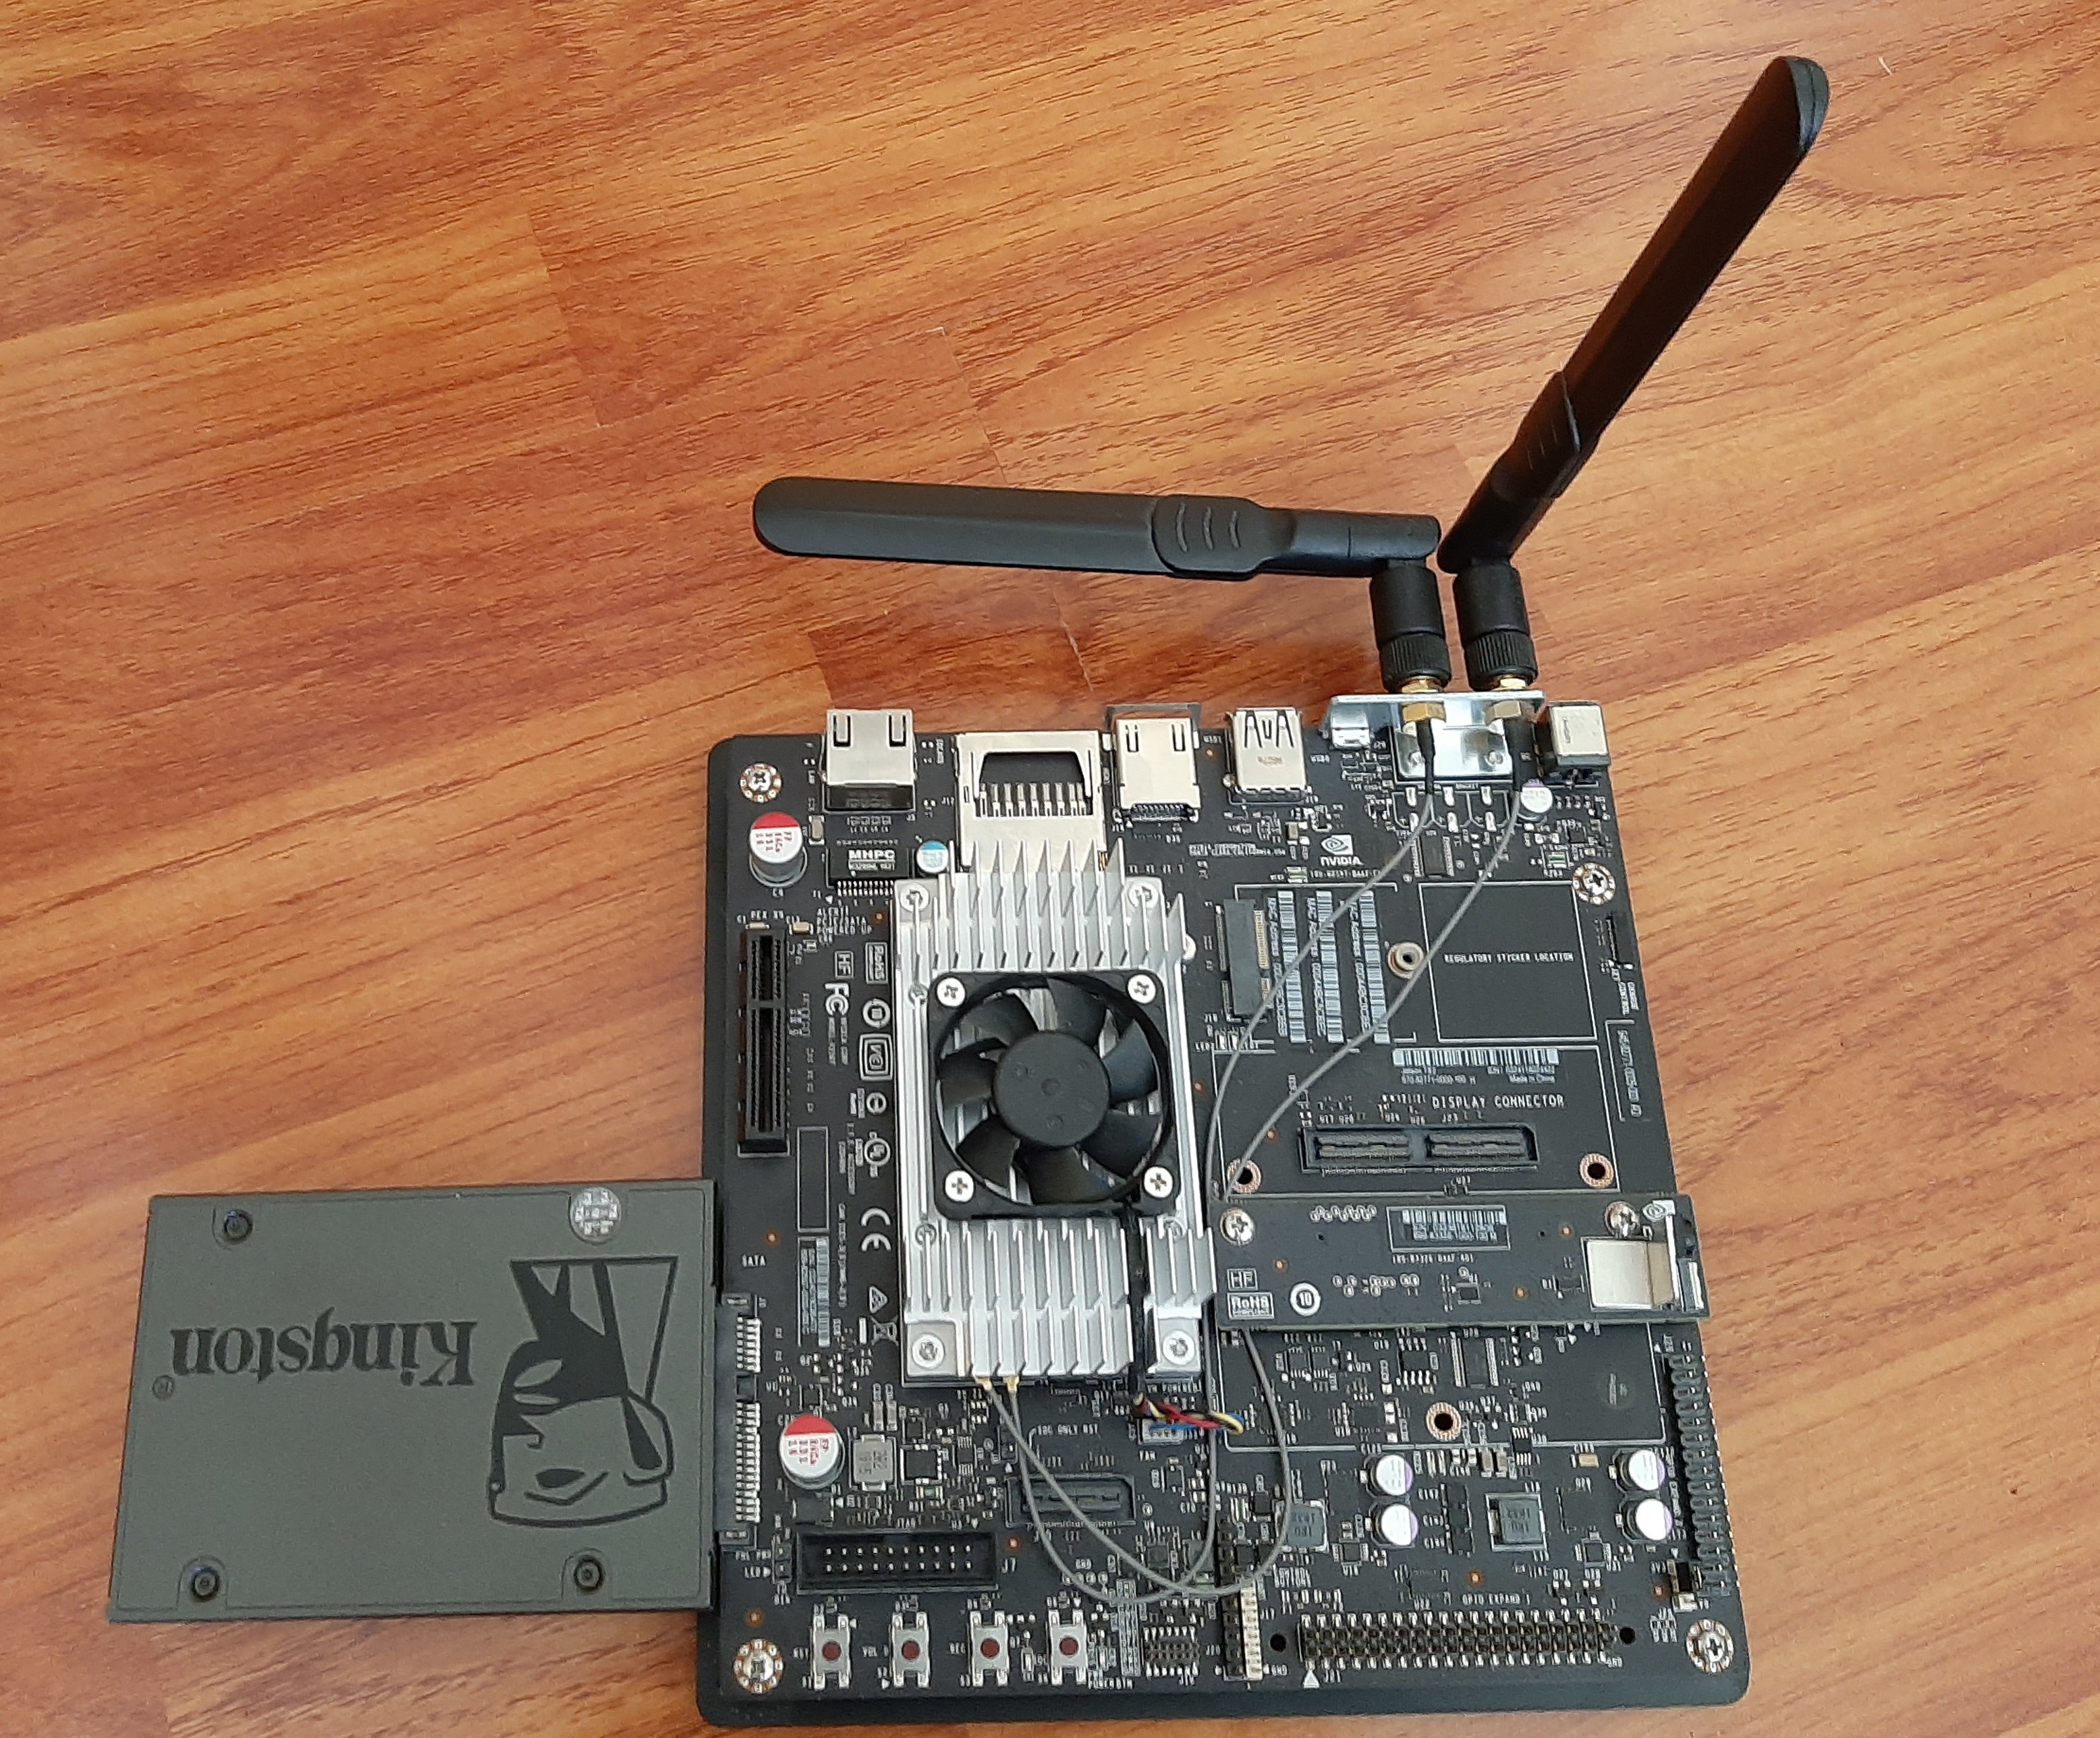
\includegraphics[width=\linewidth]{tx2_ssd}
	\end{subfigure}
	\caption{Resulting system: Jetson TX2 board and the installed SSD drive, plugged into the SATA connector.}
	\label{fig:2_mytx2}
\end{figure}
\vspace{8cm}
\subsubsection{RGBD sensor}

The vision system used in this work, the ASUS Xtion Pro Live (\autoref{fig:2_xtion}), is a USB device composed by a RGB camera and an IR emitter + sensor system, capable of retrieving depth data for each pixel on the image. This is achieved by emitting a known light pattern (\autoref{fig:2_xtion_pattern}), which reflects in the present surfaces on the scene. These reflections are captured by the IR sensor, inferring the position of the surfaces from the received distribution of the IR pattern.

\begin{figure}[h]
	\centering
	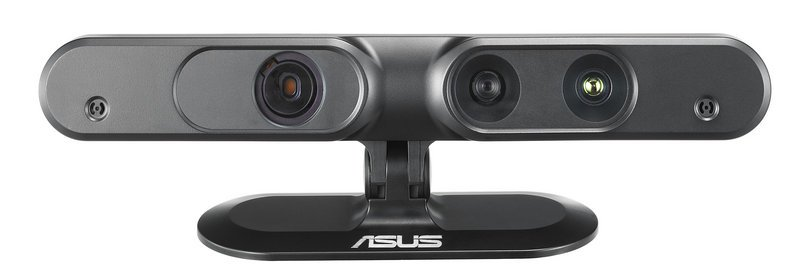
\includegraphics[width=\linewidth]{xtion}
	\caption{ASUS Xtion Pro Live}
	\label{fig:2_xtion}
\end{figure}

\begin{figure}[h]
	\centering
	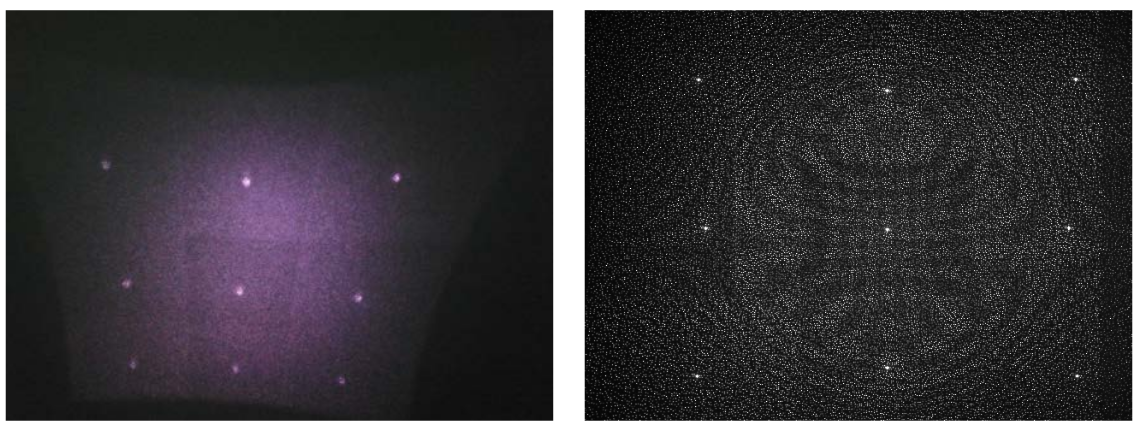
\includegraphics[width=0.9\linewidth]{xtion_pattern}
	\caption{Infrared pattern emitted by the Xtion (images from \cite{rgbd_poses}).}
	\label{fig:2_xtion_pattern}
\end{figure}

The last problem to be tackled by this device is the discrepancy caused by the different points of view of the RGB and depth sensor. However, as the distance between these two sensors is fixed and known, a \textit{registration} process can be carried on inside the device, projecting the depth data into the RGB pixels \cite{diapos_cv_registration}.\\

\begin{figure}[h]
	\centering
	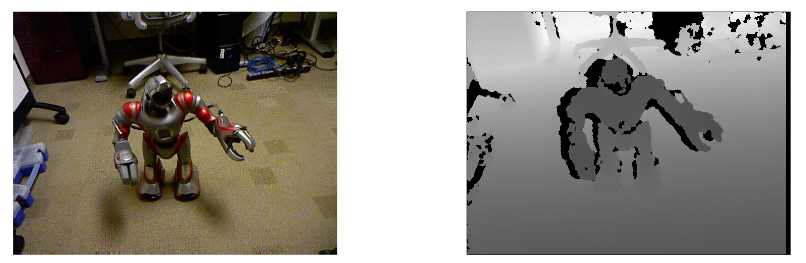
\includegraphics[width=0.9\linewidth]{xtion_discrepancy}
	\caption{Discrepancy between the RGB and depth images (image from \cite{tfg}).}
	\label{fig:2_xtion_discrepancy}
\end{figure}

The systems which implement the described design are called RGBD sensors, are suitable for robotics, as the yielded result is a point cloud, reflecting the distance from the camera for each pixel in the image. Using this, the device is capable of projecting the 2-dimensional RGB image into the 3D space by means of the depth data (\autoref{fig:2_rviz}).\\

\begin{figure}[h]
	\centering
	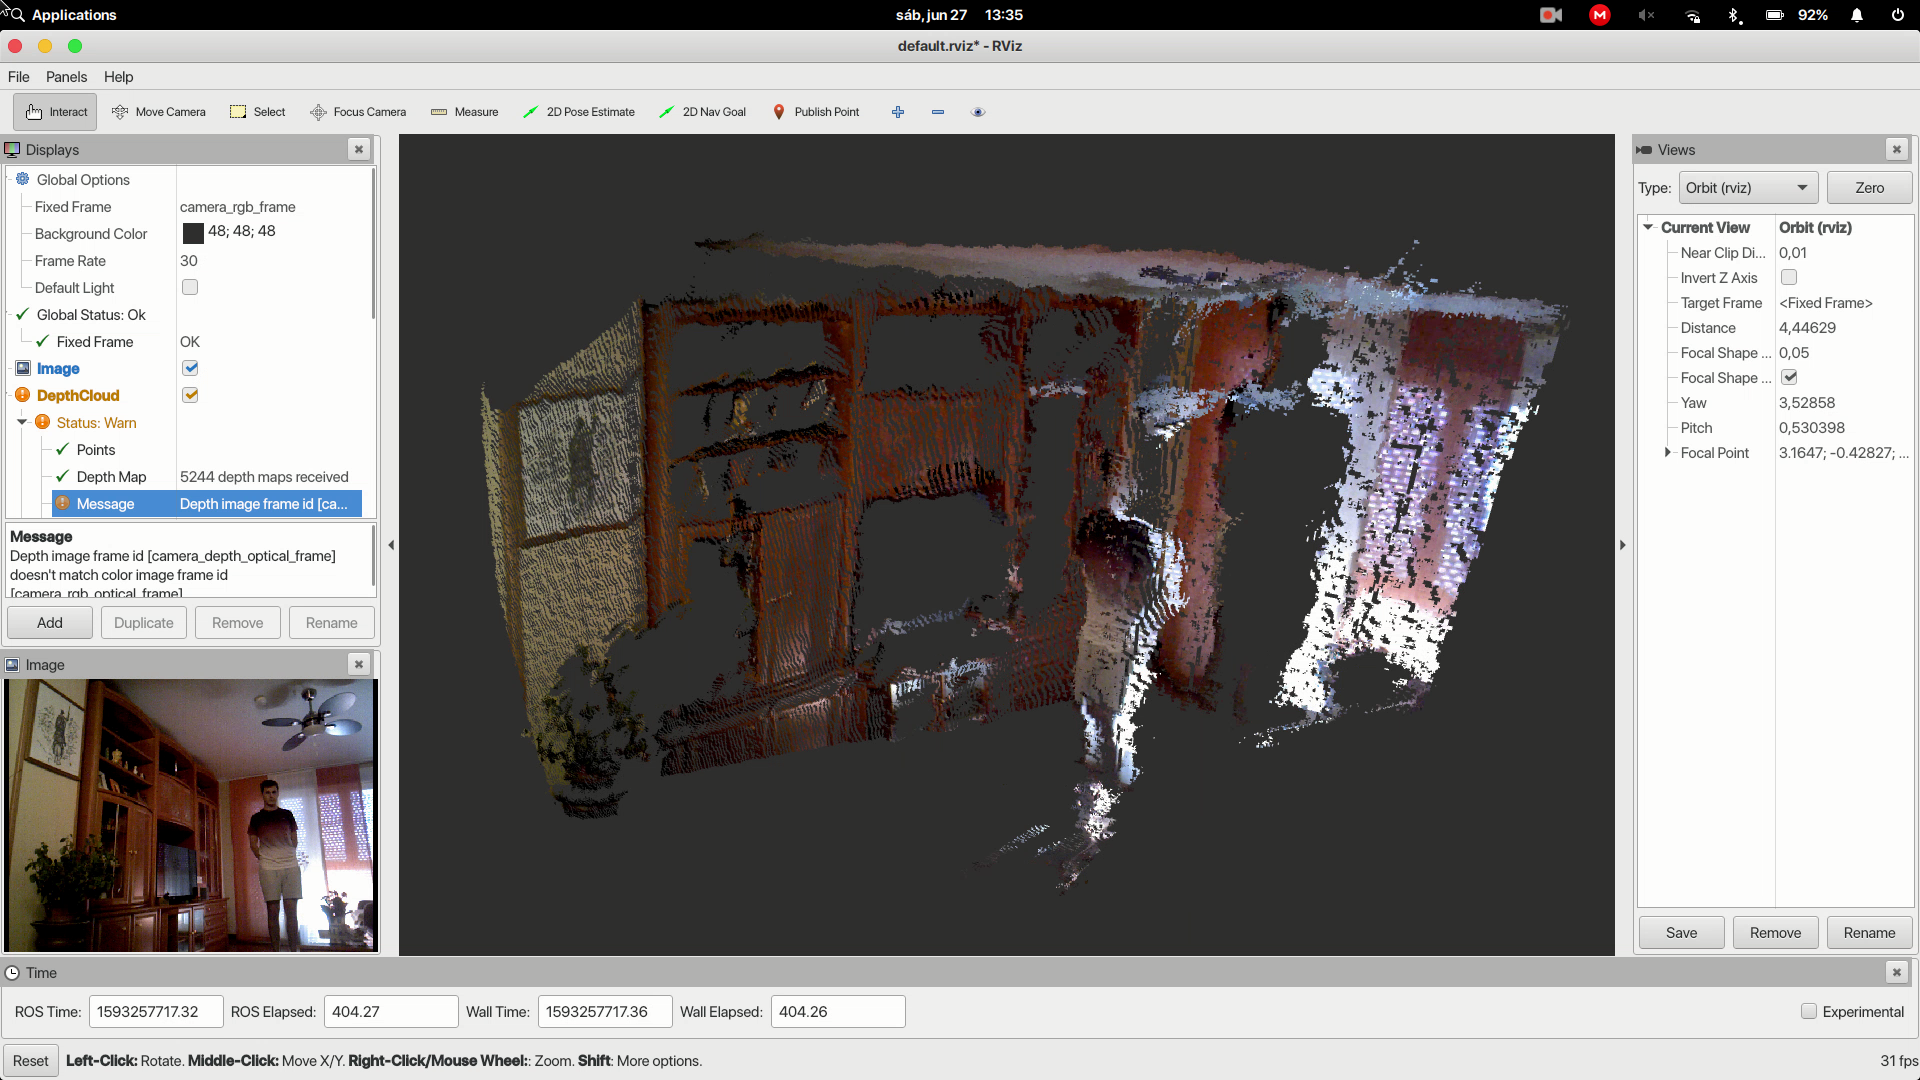
\includegraphics[width=\linewidth]{rviz}
	\caption{Visualization of the RGB image (bottom left) and the resulting point cloud projected into the 3D space (right).}
	\label{fig:2_rviz}
\end{figure}

\subsubsection{Robotic platform}
On the other hand, the robot used in this work is the Turtlebot2 educational set. It is based on a Yujinn Robotics Kobuki mobile base (\autoref{fig:2_kobuki}), which is a non-holonomic robot with 2 degrees of freedom: \textit{linear speed} and \textit{angular speed}.\\
\begin{figure}[h]
	\centering
	\begin{subfigure}[h]{0.4\linewidth}
		\centering
		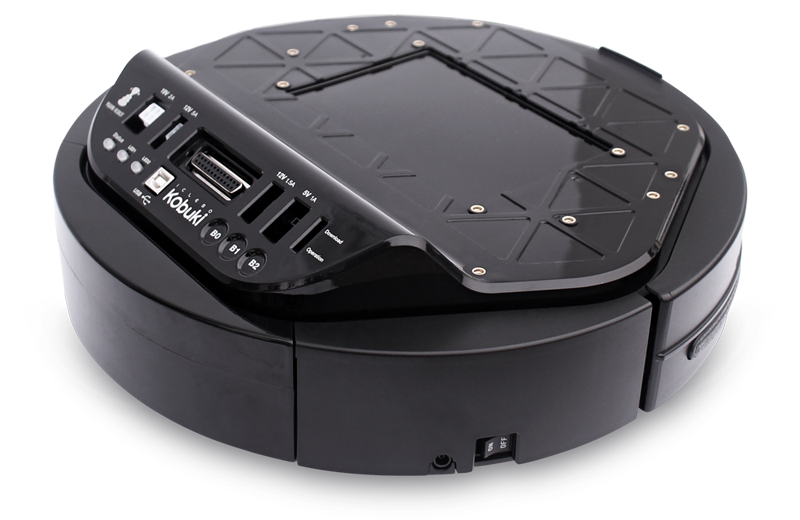
\includegraphics[width=0.9\linewidth]{kobuki}
		\caption{Appearance of the mobile base robot.}
		\label{fig:2_kobuki_appearance}
	\end{subfigure}
\begin{subfigure}[h]{0.5\linewidth}
	\centering
	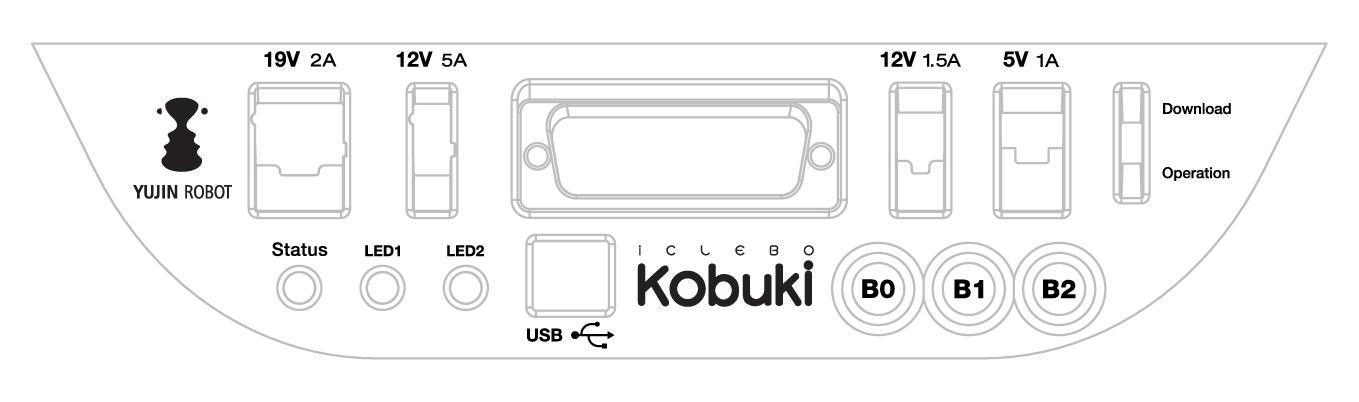
\includegraphics[width=0.9\linewidth]{kobuki_panel}
	\caption{Schematic of the connections panel of the Kobuki.}
	\label{fig:2_kobuki_panel}
\end{subfigure}
\caption{Kobuki mobile base, which carries the rest of the structure.}
\label{fig:2_kobuki}
\end{figure}

In the Turtlebot2 set, the mobile base has an attached structure, carrying the RGB-D sensor and a platform where typically a computer can be placed. This platform is useful to mount the NVIDIA Jetson device on. Additionally, as it can be seen in \autoref{fig:2_kobuki_panel}, the Kobuki panel is equipped with a 12V output, yielding up to 1.5A, which in power terms can be translated to a maximum power of 18W. As the TX2 board peak consumption is 15W, this connector is suitable to power the system up, with an additional power margin of 3W. A lookup in the Kobuki user guide \cite{kobuki_manual} allows to find the suitable Molex connector, which can then be attached to two-wire cable and a rounded connector. This provides the NVIDIA Jetson of a 12V DC supply, similar to what it would obtain from a power outlet with a transformer. As the power input is equipped with a DC voltage regulator, it accepts voltages from 5.5V to 19V (table 59 in \cite{tx2_manual}), this is a successful approach to build an \textit{autonomous} system: powering the computing board from the batteries of the robot, with enough autonomy to be powered on for several hours. The amount of time strongly depends on the usage of the motors of the mobile base, which are the most consuming component of the ensemble.\\

The final hardware setup is displayed on \autoref{fig:2_setup}, where the described components are combined to build the autonomous setup capable of running high-complexity person following algorithms.\\

\begin{figure}[h]
	\centering
	\begin{subfigure}[h]{0.45\linewidth}
		\centering
		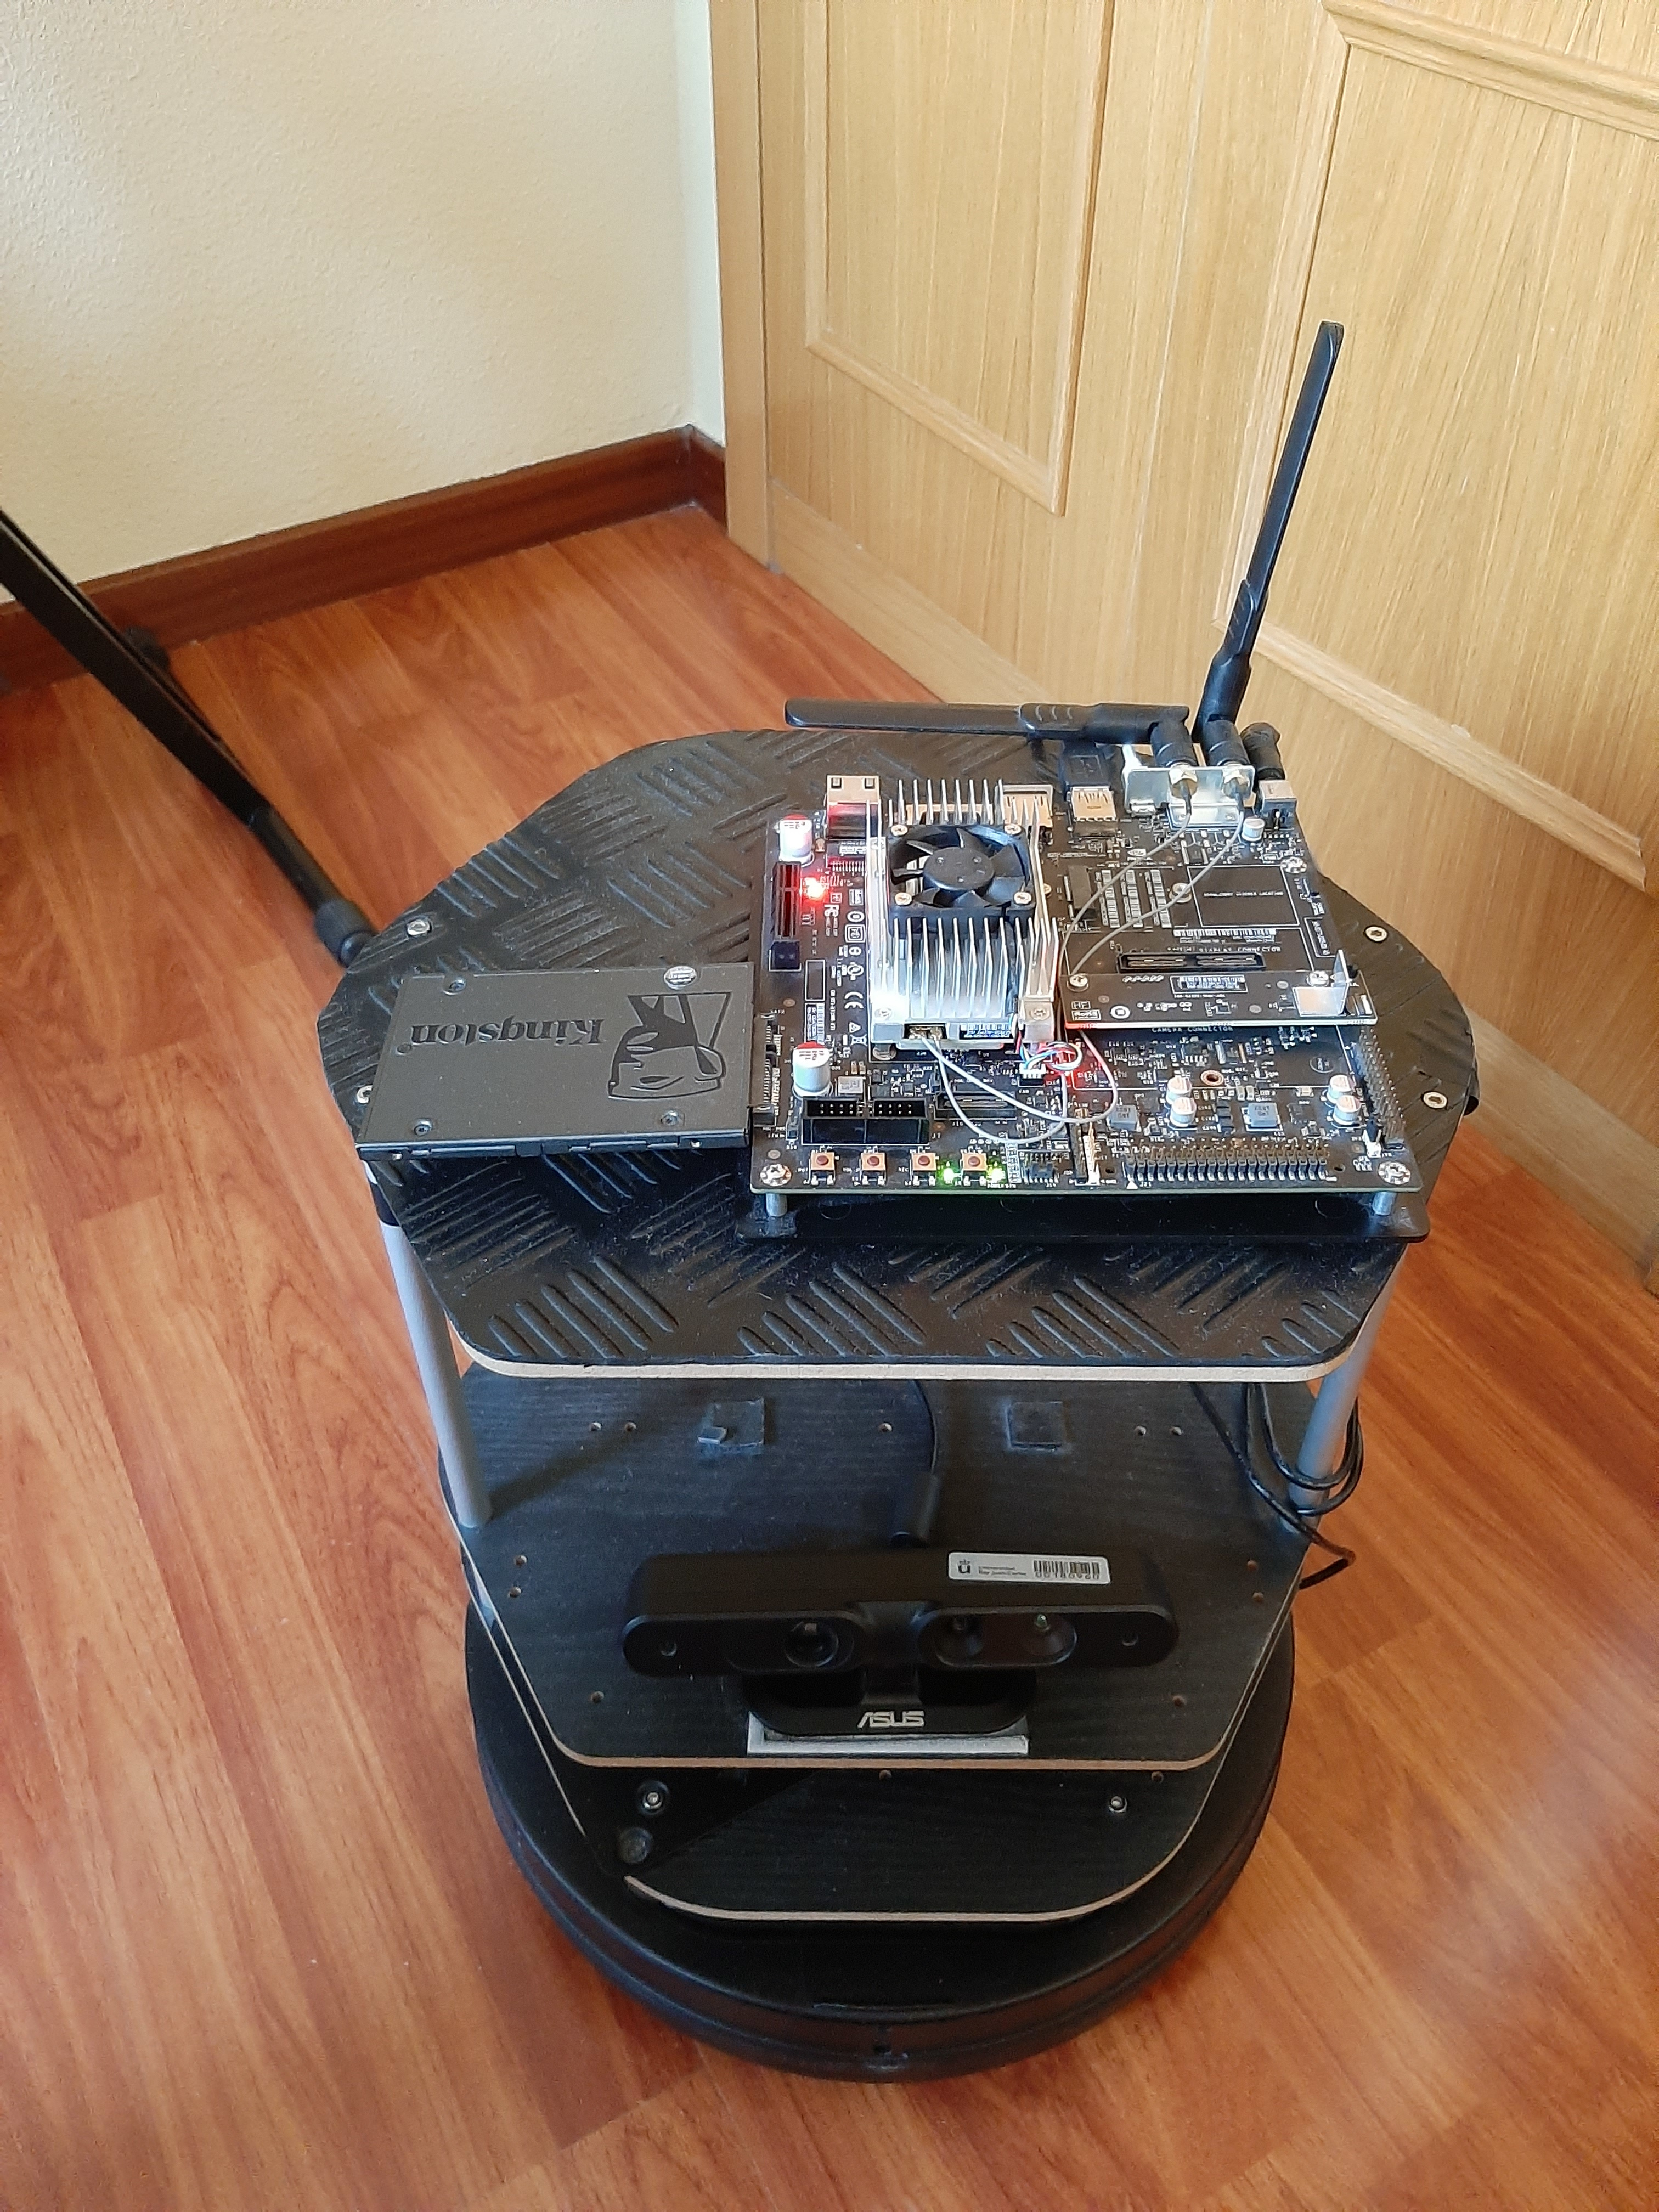
\includegraphics[width=0.9\linewidth]{setup_front}
		\caption{Front view.}
	\end{subfigure}
	\begin{subfigure}[h]{0.45\linewidth}
		\centering
		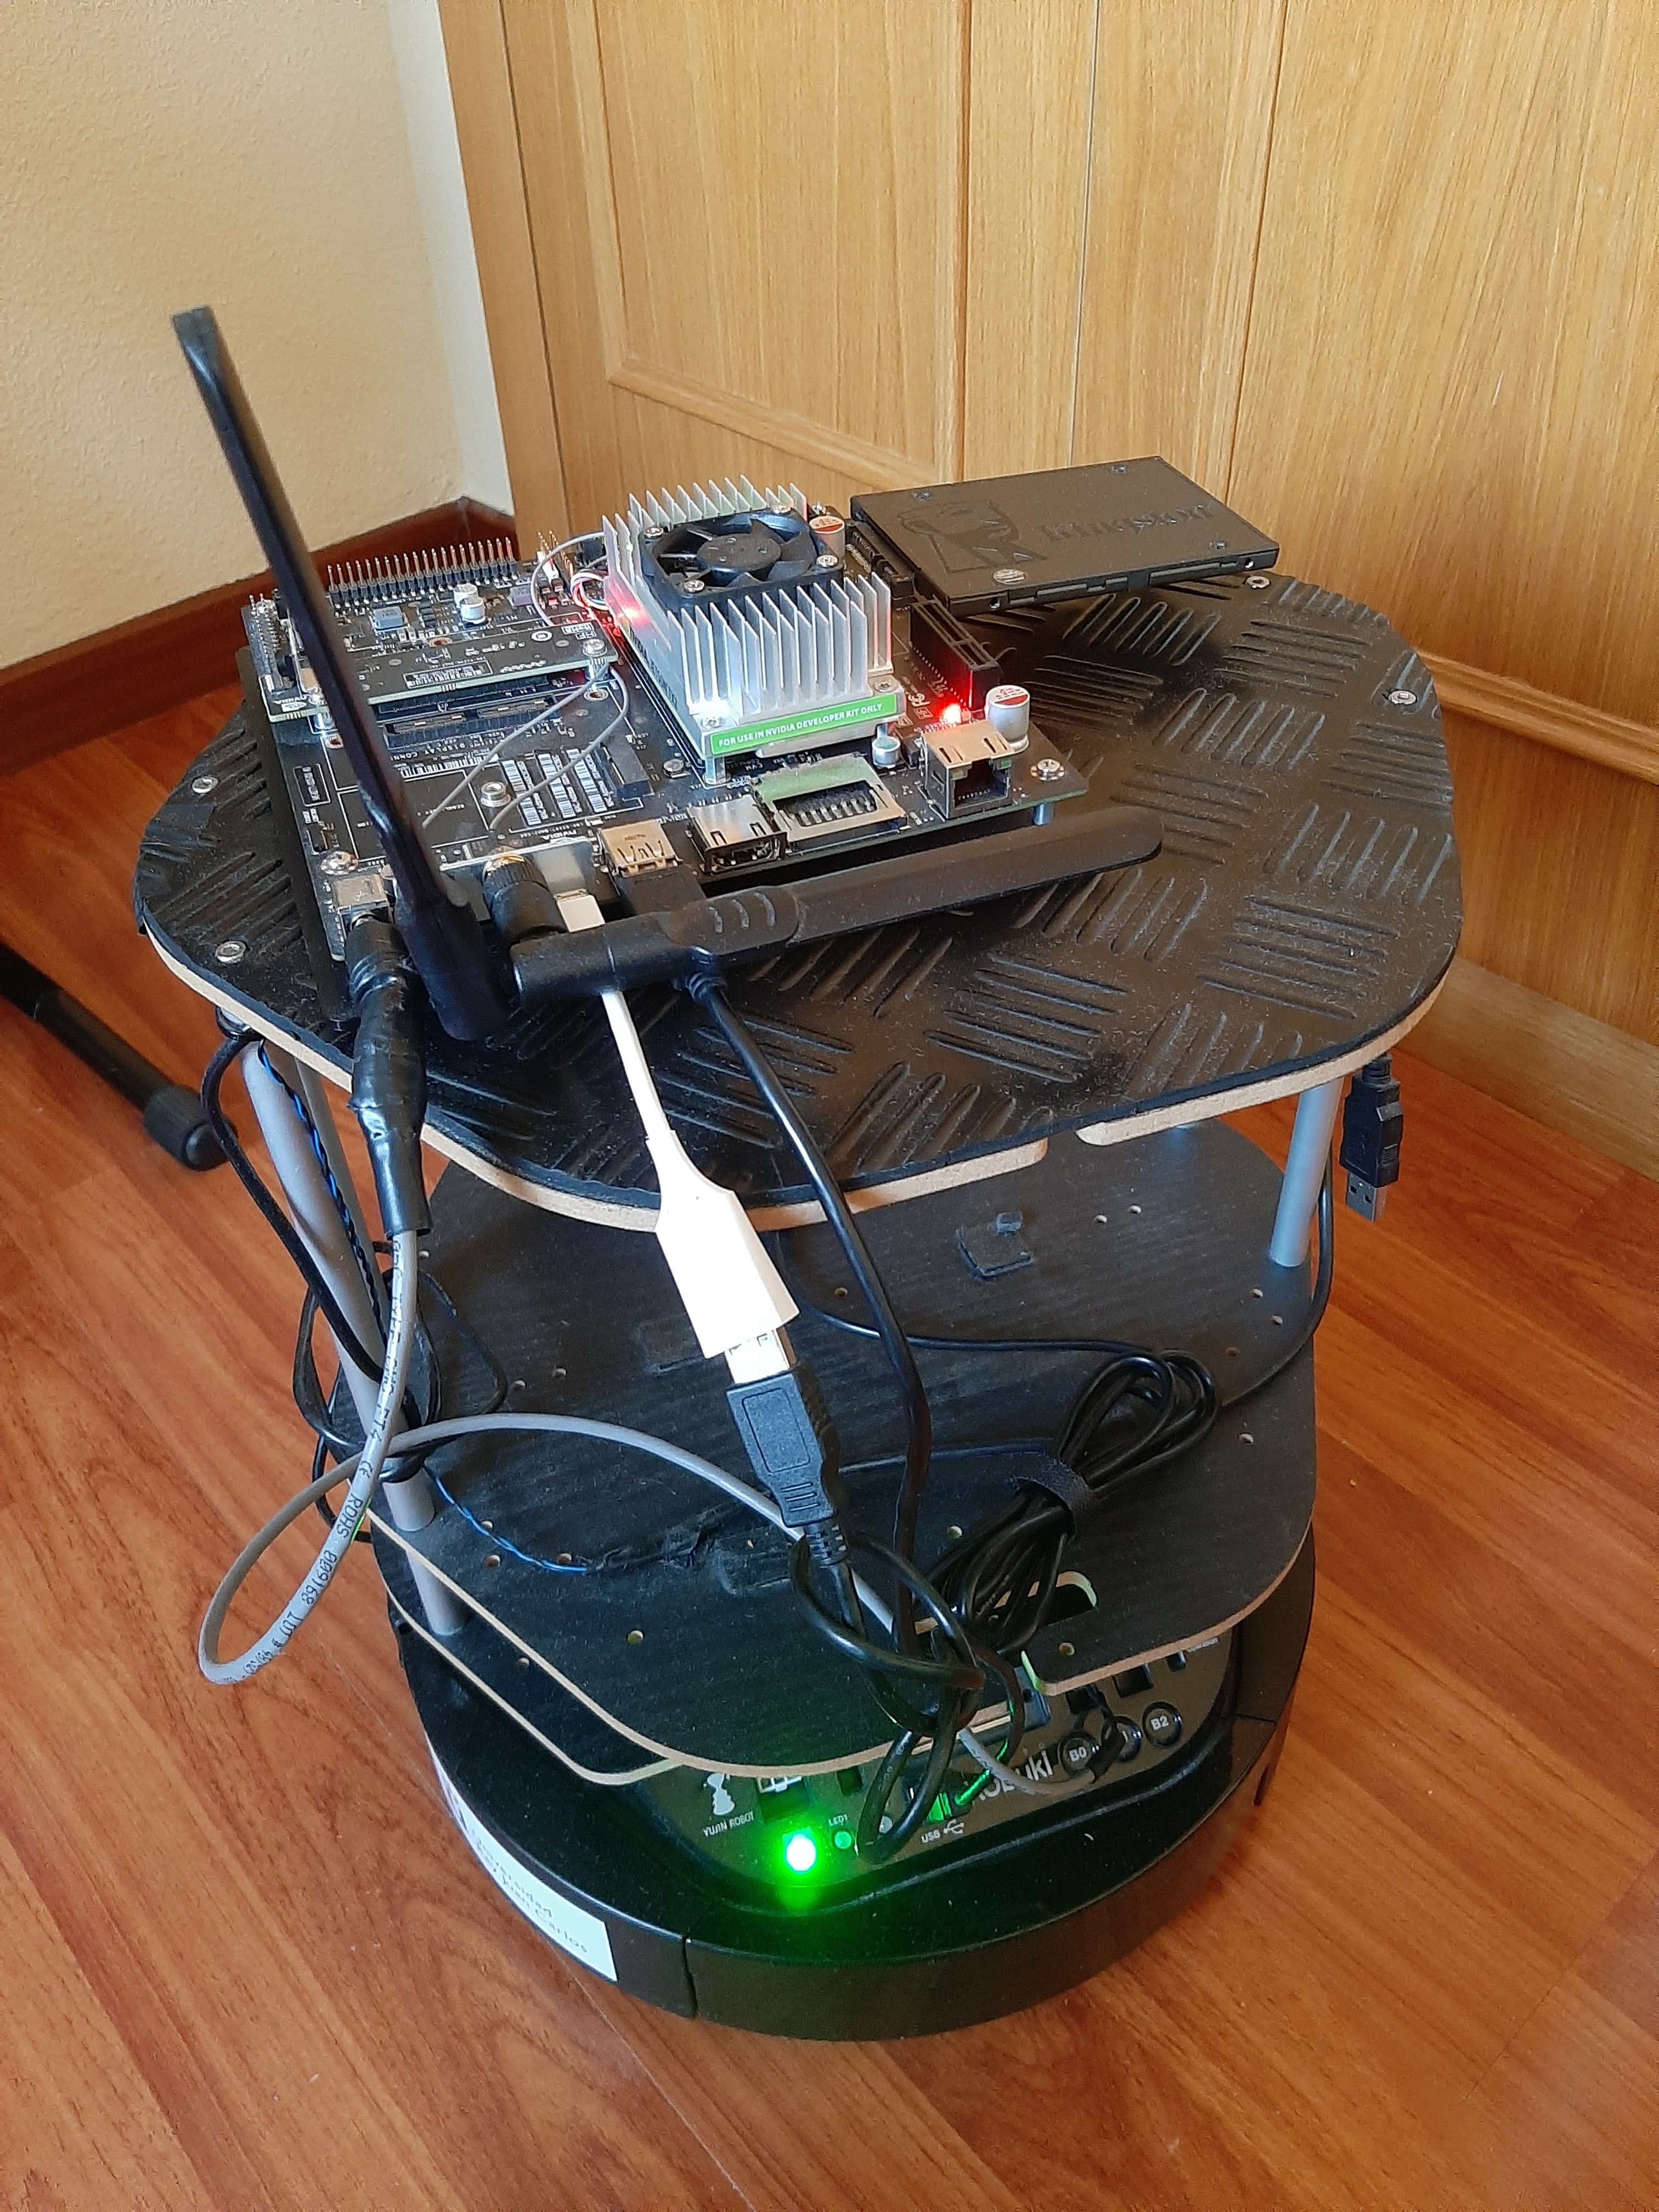
\includegraphics[width=0.9\linewidth]{setup_rear}
		\caption{Rear view.}
	\end{subfigure}
	\caption{Autonomous setup: Turtlebot2 + Jetson TX2 + ASUS Xtion Pro Live.}
	\label{fig:2_setup}
\end{figure}

\newpage
\section{Software}
\subsection{NVIDIA JetPack}
The development of our person following behavior has been tackled using exclusively open-source software. The Jetson computing board follows a tightly optimized embedded design guidelines. A tailored version of Ubuntu Linux, named NVIDIA JetPack, is developed and maintained by NVIDIA, and it is available for download and install as the board firmware. For the developed system, the version used is JetPack 4.2.2 (R32.2)\footnote{Details available on: \url{https://docs.nvidia.com/jetson/archives/jetpack-archived/jetpack-422/release-notes/index.html}}. This custom implementation includes low-level interfaces for implementing parallel computing operations (CUDA), and several optimizations SDKs (\textit{Software Development Kits}), such as TensorRT. This engine is of special interest for us, as it allows to modify the underlying implementation of a neural network, swapping certain modules (such as a convolution operation, a ReLU, or an Inception block), for a low-level optimized version of that module, allowing to greatly increase the inference speed without entailing a precision loss. Several details about these optimizations will be depicted later.\\

\subsection{Python}

This work has been developed using the Python programming language. In the previous work \cite{tfg}, the used version of the language was Python 2.7. However, as of today, that version has reached its EOL (\textit{End of Life}) date, remaining unsupported. For avoiding the obsolescence, all the code base was migrated to Python 3.6, a currently supported release, before committing any change or improvement in the functionality.

\subsection{NumPy}

NumPy\footnote{\url{http://www.numpy.org/}} (\emph{Numeric Python}) is a library for Python (written in C++), born to extend the numerical abilities of this language. It provides a powerful \texttt{ndarray} class, which allows to keep a N-dimensional collection of values/objects in a really handy way (in comparison with Python's standard \emph{lists}). It also provides a rich interface to describe the arrays (such as advanced indexing, shaping, data formatting, etc.).\\


These capabilities immediately turn this library into an excellent framework for data processing in a lower level. It allows to store and handle images and tensors on an intuitive way, providing methods to perform typical tasks such as row-wise/column-wise averaging, transposing, type conversing, or matrix slicing. The majority of these structures and methods are implemented using the C++ language, which provides a higher speed than a Python implementation.




\subsection{ROS}
This project requires hardware-software interaction, as the development board needs to read the images received by the Xtion sensor, as well as sending the final velocity commands to the robot. For this purpose, the ROS middleware is used. ROS (Robot Operating System) is \textit{an open-source, meta-operating system for your robot}, maintained by the \emph{OSRF} (\textit{Open Source Robotics Foundation}) \cite{ros-intro}. It is a framework that provides a distributed, easily-scalable environment of \emph{nodes}. These nodes are programs which run independently on the computer (or distributed over a network), so they can perform individual tasks. However, they can communicate between themselves on a synchronous way (over \emph{services}, implementing a client-server role system between nodes), or on an asynchronous way, via \textit{topics}. These topics, which rely on a standard TCP/UDP communication between sockets, are intended for an unidirectional, streaming communication, where a node can take roles: \emph{publisher} (if it is writing data inside the topic), or \emph{subscriber} (if it is reading the data that publishers are broadcasting into the topic). The data stream through the topic is not unrestricted, it must follow a ROS specific syntax, a \emph{Message} type, which is strictly defined for the communication purpose (geometry, sensoring, etc.).\\

For this project, the packages \texttt{cv\_bridge} and \texttt{openni2\_camera} have been used for handling the RGBD data. The robot can be controlled with the package \texttt{kobuki\_node}. All the software architecture is controlled by \texttt{rospy}, the interface for Python to communicate with the described ROS infrastructure.\\

Another useful feature of ROS middleware is the \textit{ROSBag} storage system. Recording a ROSBag allows to save in a single file the messages read from several topics for the time it is recorded. Later, the ROSBag can be played again to recover the messages from the topics, in the same order they were recorded. This is useful for recording video sequences from the RGBD camera, saving simultaneously the image and depth information, allowing the user to perform testing of different parameters using the exact same image source.\\

As well as in the Python case, the version of ROS used on \cite{tfg} reached its EOL date. Thus, the ROS version has been migrated as well to the currently supported release: \textit{Melodic Morenia}, which firstly provided the compatibility with Python 3. As the Jetson TX2 board is based on an ARM architecture, this upgrade has required several tweaks on the software compiling and implementation processes, which have been properly documented in the project repository\footnote{\url{https://github.com/RoboticsLabURJC/2017-tfg-nacho_condes}} for the sake of repeatability.\\


\subsection{OpenCV}
For general image processing, OpenCV (\emph{Open Source Computer Vision}) is a C++/Python/Java open-source library (natively written in C++) for Computer Vision purposes. Among the classic/\emph{state-of-the-art} methods it bundles, several functions can be found, suitable for face recognition, image stitching, eye tracking, computing homographies, establishing markers for augmented reality, etc.\\

Its general focus centers in \emph{efficiency and real-time functionality}, thank to low-level optimizations on the system hardware (i.e. integration with NVIDIA CUDA and OpenCL GPU processing libraries). Thus, the excellent performance achieved by this open source library has turned it into the \emph{de facto} standard between every kind of users (from researchers to big companies or even governmental bodies, as their website stands\footnote{\url{https://opencv.org/}}).\\

This library has been used across the entire project, on its version number 4.2.  It has been useful for diverse tasks, such as image normalization, drawing, computing local features or optical flow approximations.



\subsection{TensorFlow}


As in the previous work, the deep learning framework used is TensorFlow. This is a high-performance numerical computation library, strongly focused on parallel computing, typically carried on by GPUs or processing clusters. This library is a state-of-the-art tool to deploy deep neural networks because of its efficiency. Besides of training/running a neural model, this library allows to load a pretrained model from a storage device, by means of a \textit{frozen graph} file. The information contained in the file are both the network definition and the weights of the nodes.\\

Additionally, a binding component called \texttt{TensorFlowRT/TRT} have been used to implement the low-level optimizations on the TensorFlow neural engines, as it will be depicted later.



\section{Design}
\label{sec:2_functional_architecture}
The software implemented in this work has been split into two main components or modules, namely the \textit{perception} module and the \textit{actuation module}, which can be observed in \autoref{fig:2_functional_architecture}.

\begin{figure}[h]
	\centering
	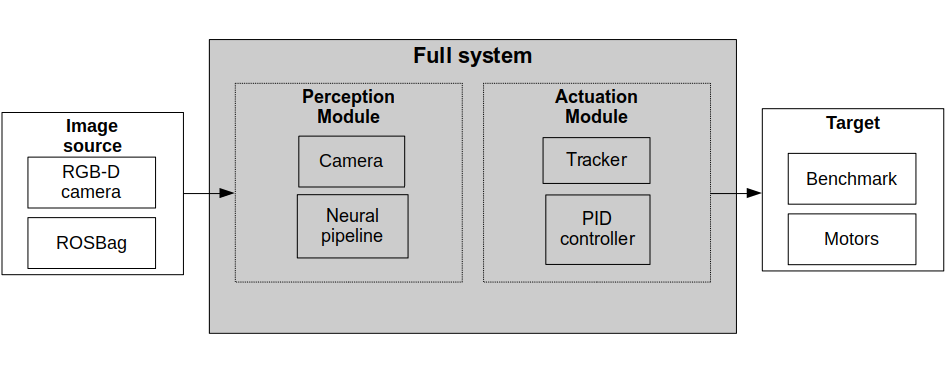
\includegraphics[width=0.7\linewidth]{functional_architecture}
	\caption{Functional architecture of the developed work, showing the two main blocks.}
	\label{fig:2_functional_architecture}
\end{figure}

These two modules cope with specific tasks on an independent manner, as it will be depicted in the following subsections:
\newpage
\subsection{Perception Module}
This module encompasses what the robot perceives from its sensors (the camera, in this case), and the processing performed to the images in order to determine the location of the person to be followed.
\subsubsection{Camera}
As it was described before, the Xtion device yields two simultaneous images: an RGB image and a depth image. The ROS controller for the camera, OpenNI2\footnote{\url{https://structure.io/openni}}, fetches the image and registered depth map from the camera, making this information available through several ROS topics. As ROS follows a \textit{publisher-subscriber} semantics, once the driver is up and running, any application may subscribe to the topics in order to receive all the published messages. In our \textit{Camera} module, two subscribers are deployed to retrieve the latest (RGB, depth) pair on an asynchronous way. These images are then converted into the standard image format in the OpenCV library, and they are ready to be used by other components. Additionally, in order to be able to perform objective testing and benchmarks, the Camera module is able to retrieve the images from a recorded ROSBag instead of the online camera. This is useful to obtain objective metrics of another components of the software on unit tests, as the ROSBag ensures that exactly the same images are used regardless the tested system.\\

The implemented \textit{Camera} module abstracts this condition, allowing to apply the system on an \textit{online} source (camera) or an \textit{offline} source (recorded ROSBag), on a transparent adaptation to the rest of the system. Whenever a new (RGB, depth) pair is required, the \textit{Camera} module will serve the latest available image from the specified source.\\
\vspace{1cm}
\subsubsection{Neural pipeline}

On the other hand, the received images are passed through an ensemble of neural networks, which provide the capability of detecting the persons in the scene, as well as identifying which one is the one to be followed. As it was studied in \autoref{sec:1_sota}, the most powerful and robust approaches are achieved nowadays using deep learning. Thus, the complex problem of determining the identity and location of the person of interest has been decomposed into three tasks, which are all addressed using the corresponding deep learning techniques:
\begin{enumerate}
	\item \textbf{Person detection:} the generalized \textit{object detection} task (\autoref{fig:2_person_detection}) is a common challenge in computer vision. The existing solutions use object detectors similar to those explained in \autoref{sec:1_sota}, which are typically trained with large image datasets. The classes these models are capable to detect contain the \textit{person} class. Thus, as it was demonstrated in \cite{tfg}, a deep object detector can be utilized for detecting persons inside the image. On this work, several models have been tested, varying the base network architecture and depth. As one of the objectives of the system is to work on a portable (low-power) system, only the architectures which yield a good performance with a sufficiently low inference time are considered. The two most suitable models for this purpose are SSD \cite{ssd} using a MobileNet \cite{mobilenet} for feature extraction, and YOLOv3 \cite{yolov3} on its tiny version\footnote{The usage of the tiny version of YOLOv3 is due to issues with the limited memory on the Jetson TX2 board. The full model was tried unsuccessfully, as it requires more memory than the available one on a typical execution.}. These models are previously trained and publicly available on the TensorFlow Model Zoo \cite{model_zoo} and on repositories hosted on GitHub\footnote{\url{https://github.com/mystic123/tensorflow-yolo-v3}}. In-depth tests have been developed to compare the performance of these two models, which can be found in \autoref{chap:3_results}. The previously developed work \cite{tfg} only supported SSD-based detectors, however, the object detection component of the program has been upgraded and it features YOLOv3 support as well, making it available through the configuration file specified on launch.
	
\begin{figure}[h]
	\centering
	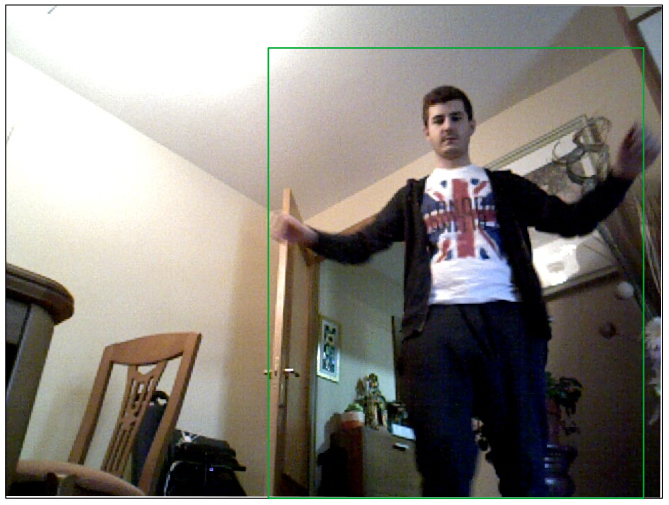
\includegraphics[width=0.5\linewidth]{person_detection}
	\caption{Example of a person detection task.}
	\label{fig:2_person_detection}
\end{figure}
	
	\item \textbf{Face detection:} as in the previous point, the problem can be addressed using an object detection neural network. However, the previously deployed models are not capable of detecting faces. As the system is power-limited, looking for another multi-class model could be considered as an overshooting solution that the system is not able to handle at the same time the other model is deployed. Thus, one feasible solution is to use a single-class detection system. The network trained in \cite{faced} implements a two-stage neural network capable of detecting faces. As it was depicted in \autoref{sec:1_sota}, this detector is based on YOLO, which ensures a high-speed and efficient detection deployed using a class-specific neural network, which is lighter than a multi-class detection system. The repository where the project is hosted contains a video sequence comparison comparing the accuracy of this system against a classical Haar cascade approach \cite{violajones}.  Chapter \ref{chap:3_results} contains data and captions of this sequence to show the superior performance for the face detection issue.
	
	\item \textbf{Face identification:} Once the face of a person has been retrieved, it can be used as a distinguishing feature for determining their identity. As the basis of this work is to take advantage of deep learning power, a neural system has been selected to perform this task too. For this purpose, \textit{FaceNet} (described on \autoref{sec:1_facenet}) has been deployed in order to perform identification, using a publicly available implementation in TensorFlow\footnote{\url{https://github.com/davidsandberg/facenet}}. As a result, the image of a face is transformed into a 128-dimensional vector: its projection or \textit{embedding}. This transformation is learned after a triplet-loss training process, which separates different faces as much as possible, while projecting similar faces as close as possible. As it can be seen on \autoref{fig:1_faces_poses}, this can be use to obtain similar projections when two images of the same face are evaluated, despite different lighting conditions (as a channel-wise normalization step is performed before passing the image through the network).
	
\end{enumerate}

To sum up, this ensemble of 3 neural networks provides a sequential pipeline to obtain \textit{person locations, face detections and face projections} from a single image, taking advantage of the flexibility and robustness that deep learning methods offer, in order to address three different problems on an efficient way. Its functionality has been depicted in \autoref{fig:2_neural_pipeline}.\\


\begin{figure}[h]
	\centering
	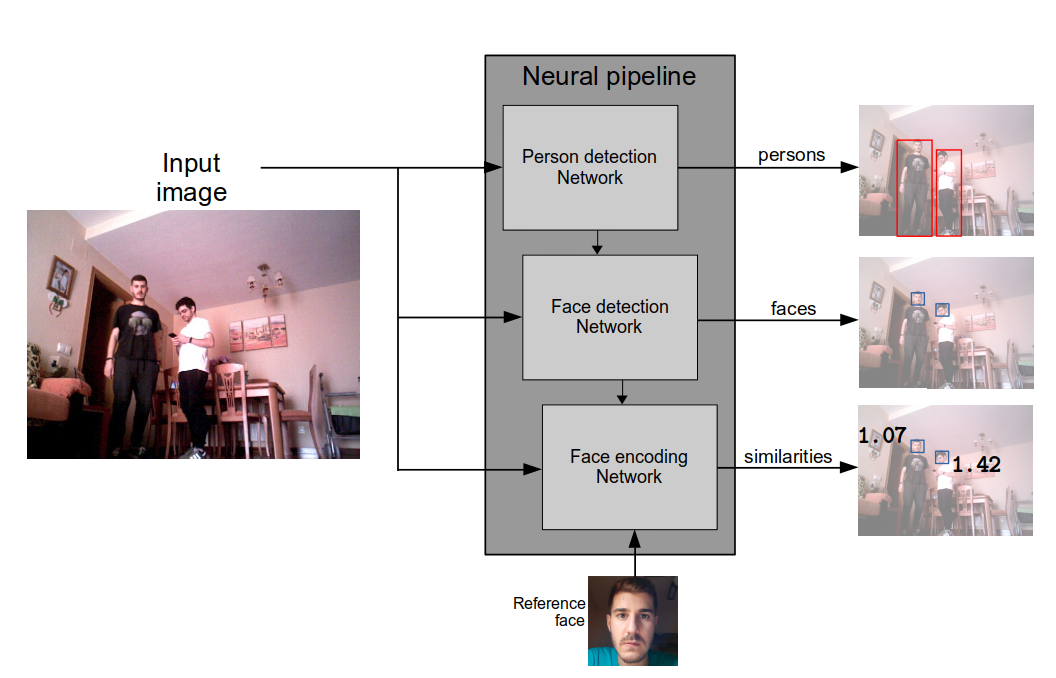
\includegraphics[width=\linewidth]{neural_pipeline}
	\caption{Neural pipeline, showing the cascade of the three neural networks used to output persons, faces and similarities with the reference face.}
	\label{fig:2_neural_pipeline}
\end{figure}

\vspace{1.7cm}

Once the inference pipeline has been designed and implemented, it can take advantage of the optimization libraries present in the Jetson TX2 board, using TensorRT for this purpose. Using this library, several segments from the architecture of a given network can be modified according to certain parameters:

\begin{description}
	\item[MSS (\textit{Minimum Segment Size})] the threshold above which a segment is selected to be replaced by the TensorRT optimization. Increasing this value makes the optimizer more selective, in order to optimize only the heaviest segments of the network. A low value aims to optimize smaller segments, although this may cause an excessively high overhead, causing the resulting graph to run slower than the original one. 
	\item[MCE (\textit{Maximum Cached Engines})] TensorRT keeps a cache of engines on runtime, with the purpose of reducing the time spent for loading them into the GPU. This parameter modulates the amount of engines kept in that cache, in case the available memory to establish the cache is limited.
	\item[Precision mode] typically, the weights and parameters of the trained neural networks are handled as 64-bit floating point numbers. A reduction in the precision to 32-bit or 16-bit achieves very similar results, making the operations much lighter as the precision mode is reduced by $\frac{1}{2}$ or $\frac{1}{4}$. A more daring approach reduces the precision up to 8-bit integers, performing an additional \textit{quantization} step since the range will be limited to 256 values. The quantization step analyzes the segment, computing the numeric range of its weights. This range is typically narrow enough to perform a 8-bit quantization, mapping the high-precision weights into a range composed of 256 values between the minimum and maximum values of the weights.
\end{description}

An experimental tuning of these parameters has been performed in \autoref{chap:3_results}, looking for an optimization of the inference time and taking into account that the enhanced models of the three neural networks have to share the limited available memory on board. Thus, care has been put into the memory footprint that an excessive runtime optimization might cause, as this leads to a high time penalization if the system cache is utilized to store the models.\\


The \textit{Camera} and \textit{Neural} components form the \textit{Perception} module, responsible of retrieving the external image and apprehend the underlying information from the image: position and identity of the person to be followed. This information serves as input to the actuation module, explained below.


\subsection{Actuation Module}

The second module of the system addresses the actuation task: once the external stimuli have been acquired and processed, an action has to be performed in order to move the robot towards its goal. As the final objective of the system is to follow a person, these movements have to be reactive, happening as soon as possible whenever the person changes their position.\\

\subsubsection{Motion Tracker}

The previously depicted \textit{Neural} component outputs reliable inferences with a certain refresh rate, namely $k$, which can reach a relatively high value depending on the current load and power profile in the development board. If $k$ is too high, the system may run the risk of suffering an important delay when the movement is performed. This may lead in unsteady movements, with a higher probability of losing the reference person. To avoid this, a \textit{Tracker} component is added to the system. Its functionality is to be able to \textit{estimate} the person movement along $k$ frames, while the neural pipeline is performing detections. This way, currently detected persons can be tracked along the image while they wander, until the neural ensemble outputs the latest predictions, which determine the true new position of the persons. To fulfill this requirement, the tracking method has to be able to run at a higher rate than $k$, preferably with a considerably lower inference time. This way, the system counts on a slow, reliable detection system supported by a fast estimation system, devoted to guess the movements between detections. This tracker has been situated in the \textit{Actuation} module. This is because it is focused on keeping the position of the person updated, in order to move towards them as fast as possible. This task is performed without a detection algorithm behind, just moving the box using the estimated optical flow, which is a completely different task of the \textit{Perception} module one. For this reason, it has been separated from the neural pipeline and placed in the \textit{Actuation} module.\\

The method chosen for this purpose is a \textit{Lucas-Kanade} visual tracker \cite{diapos_cv_motion_estimation}.  This technique estimates the \textit{motion field} between the images taken in two time instants, addressing the problem using a differential approach \cite{lucas_kanade}:

The basis relies on the fact that in a video sequence, for small changes in space and time, the intensity remains constant inside a certain pixel neighborhood:

$$
\mathbb{I}(\mathbf{x}, t) = \mathbb{I}(\mathbf{x} + \Delta \textbf{x}, t + \Delta t)
$$

Using a \nth{1} order Taylor series approximation and algebra, the \textit{optical flow equation}, $f$, can be found\cite{lucas_kanade_tutorial}:

$$
f_xu+ f_yv + f_t = 0
$$
where
$$
f_x = \frac{\partial f}{\partial x} ; f_y = \frac{\partial f}{\partial y}\\
$$
$$
u = \frac{dx}{dt} ; v = \frac{dy}{dt}
$$

$f_x$, $f_y$ and $f_t$ represent the image gradients with respect to the space and time, respectively, and $(u, v)$ represents the movement vector of the scene.

\begin{figure}[h]
	\centering
	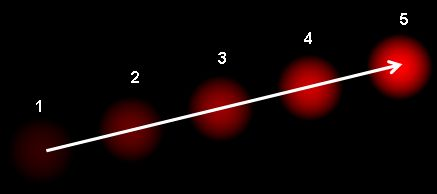
\includegraphics[width=0.6\linewidth]{optical_flow}
	\caption{Optical flow for different time instants. Image from \cite{lucas_kanade_tutorial}.}
	\label{fig:2_optical_flow}
\end{figure}

At this point, the resulting system is under-determined as the problem presents 1 equation with 2 unknown variables. Lucas-Kanade algorithm addresses this problem taking advantage of one of the previous assumptions: as the pixel intensity remains constant for a pixel neighborhood, one can expect the same movement on neighboring pixels: these will share a common $(u, v)$ movement vector (typically, a small square or circular neighborhood is assumed). Assembling together those equations results in an over-determined system, where a \textit{Least-Squares} solution yields the best-fitting movement vector $(u,v)$ for that neighborhood, allowing to have a local estimation for the movement in that area:

\begin{equation}
\begin{bmatrix} u \\ v \end{bmatrix} = \begin{bmatrix} \sum_{i}{f_{x_i}}^2 & \sum_{i}{f_{x_i} f_{y_i} } \\ \sum_{i}{f_{x_i} f_{y_i}} & \sum_{i}{f_{y_i}}^2 \end{bmatrix}^{-1} \begin{bmatrix} - \sum_{i}{f_{x_i} f_{t_i}} \\ - \sum_{i}{f_{y_i} f_{t_i}} \end{bmatrix}
\label{eqn:2_lk_ls}
\end{equation}

The computation of \autoref{eqn:2_lk_ls} can be efficiently performed with high-performance libraries, such as \textit{NumPy} or \textit{TBB}, which ensure a fast execution of the estimation. This makes Lucas-Kanade estimation an efficient approach to compute the optical flow in tasks such as image registration, video stabilization or depth computation in stereo vision systems. This technique is implemented in the \textit{OpenCV} library through the method\\ \texttt{cv2.calcOpticalFlowPyrLK}, which evaluates the image on a pyramid of scales to improve the robustness. This method offers a set of tunable parameters to detect the new position of the corners:

\begin{description}
	\item[\texttt{winSize}] size of the window to perform the LS solution.
	\item[\texttt{maxLevel}] number of additional scales to evaluate the image on a pyramidal scale sequence.
	\item[\texttt{criteria}] flags to determine the stop condition on the iterations of the algorithm.
\end{description}

However, in the case of study of this work, a calculation of the motion field on the entire image would be considered overshooting (besides of a dangerously slow task for a real-time system), as the objective is not to compute the entire optical flow. The estimation can be limited to the pixels inside and surrounding the persons in the scene. Furthermore, one can notice the existence of more informative regions inside the person than others, given its texture: typically object \textit{corners} will be the best choice to be tracked \cite{diapos_cv_features}, given their easiness to be identified and the fact that they provide more motion information than another areas (aperture problem). In order to detect these corners, a Harris corner detector can be used, analyzing the eigenvalues inside different 2-D windows inside the image. A \textit{corner response} can be computed, yielding a score depending on the eigenvalues and their ratio:
$$
R = \det M - k(\operatorname{trace}(M))^2
$$
with k being an empirical constant $k=0.04-0.06$, and $M$ being the diagonal matrix resulting of the singular value decomposition of the current window.

The value of $R$ determines the decision taken of the window containing a corner.

A modification of this algorithm, the \textit{Shi-Tomasi} corner detector was published on \cite{shi_tomasi}, improving the performance of the corner detector by changing the corner response computation to:
$$
R = \min(\lambda_1, \lambda_2)
$$

taking the window as a corner if $R$ is greater than a given threshold. The scoring diagrams for determining the corner response on the two depicted methods can be observed in \autoref{fig:2_harris_vs_shi}. One advantage of this methodology is its invariance to rotation, as it works using the eigenvalues, that automatically align to the most variant directions. However, one important thing to mention as a flaw is the variance to scale: the relative size of the corner with respect to the window size has influence on the eigenvalues.\\

Other methods for corner detection are widely used in state-of-the-art developments, such as SIFT \cite{sift} or FAST \cite{fast}. However, according to the evaluation among several corner detectors on \cite{corner_detectors} reveals that the Harris/Shi-Tomasi approach yields a more reliable result for this purpose, while taking a low time to execute: it takes around 25 ms to evaluate the $640\times 480$ image from the Asus Xtion, which makes the tracking module to run 5x faster than the neural pipeline.

\begin{figure}[h]
	\centering
	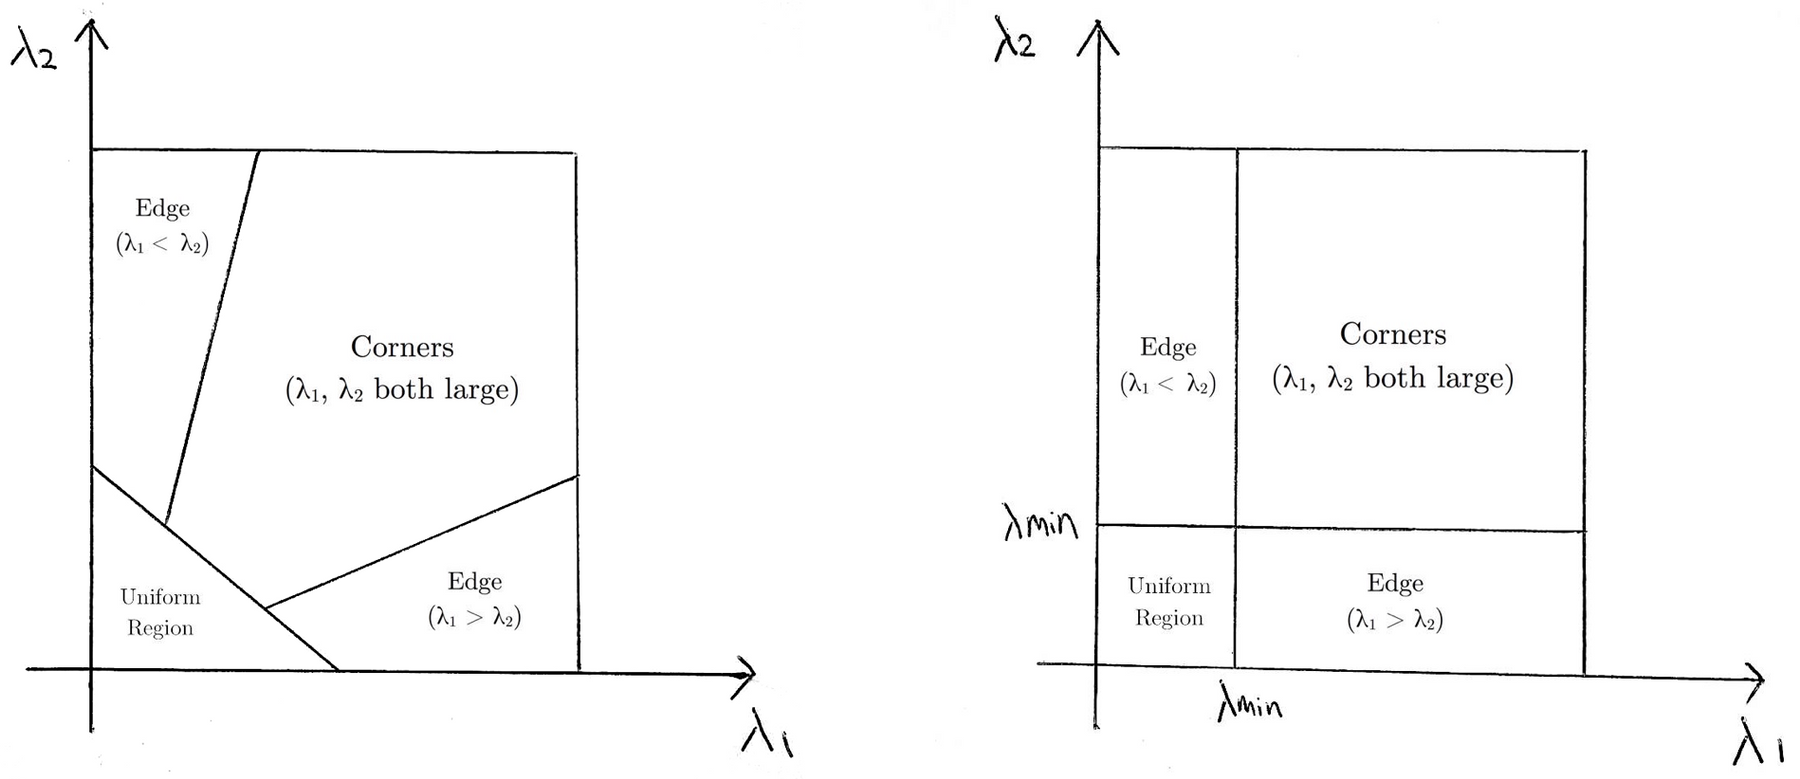
\includegraphics[width=0.8\linewidth]{harris_vs_shi_boundaries}
	\caption{Corner response $R$ scoring functions on $\lambda_1-\lambda_2$ on the Harris (left) and Shi-Tomasi (right) detectors (source:\cite{nanonets_optical_flow}).}
	\label{fig:2_harris_vs_shi}
\end{figure}

\begin{figure}[h]
	\centering
	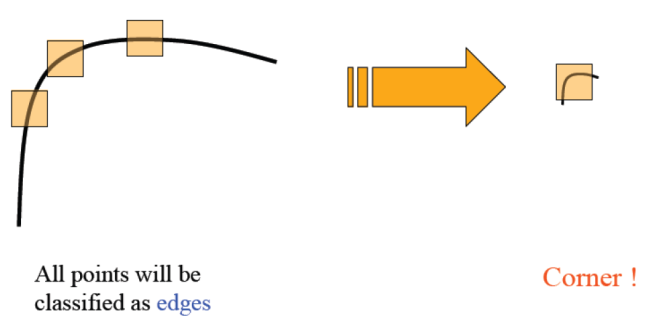
\includegraphics[width=0.8\linewidth]{harris_scale_variance}
	\caption{Scale variance of this method, where the size of the corner with respect to the \texttt{winSize} jeopardizes the eigenvalues.}
	\label{fig:2_harris_scale}
\end{figure}

Using this method returns what the authors call the \textit{good features to track}, namely, the best N corners of the image or region provided.

 This method is implemented in the \textit{OpenCV} library through the method \texttt{cv2.goodFeaturesToTrack}, which offers a set of tunable parameters to extract corners from a given image:
 \begin{description}
 	\item[\texttt{maxCorners}] maximum number of corners to be found.
 	\item[\texttt{qualityLevel}] multiplicative factor for the $R$ of the best corner. A corner response below $\text{qualityLevel}\cdot R_{max}$ will be discarded.
 	\item[\texttt{minDistance}] minimum euclidean distance between the selected corners.
 	\item[\texttt{blockSize}] size of the pixel block to compute the eigenvalues.
 \end{description}

The combination of these two methods provides a fast methodology to estimate the movement of a region using exclusively algebraic calculations on the pixel intensities. As these computations are bounded in complexity, the iteration time is around 5x faster than the neural pipeline. Thus, the simultaneous combination of both algorithms allows to track the movements of the persons during $K$ frames, until the next neural update arrives. This is shown in \autoref{fig:2_tracker_demo}.\\

\begin{figure}[h]
	\centering
	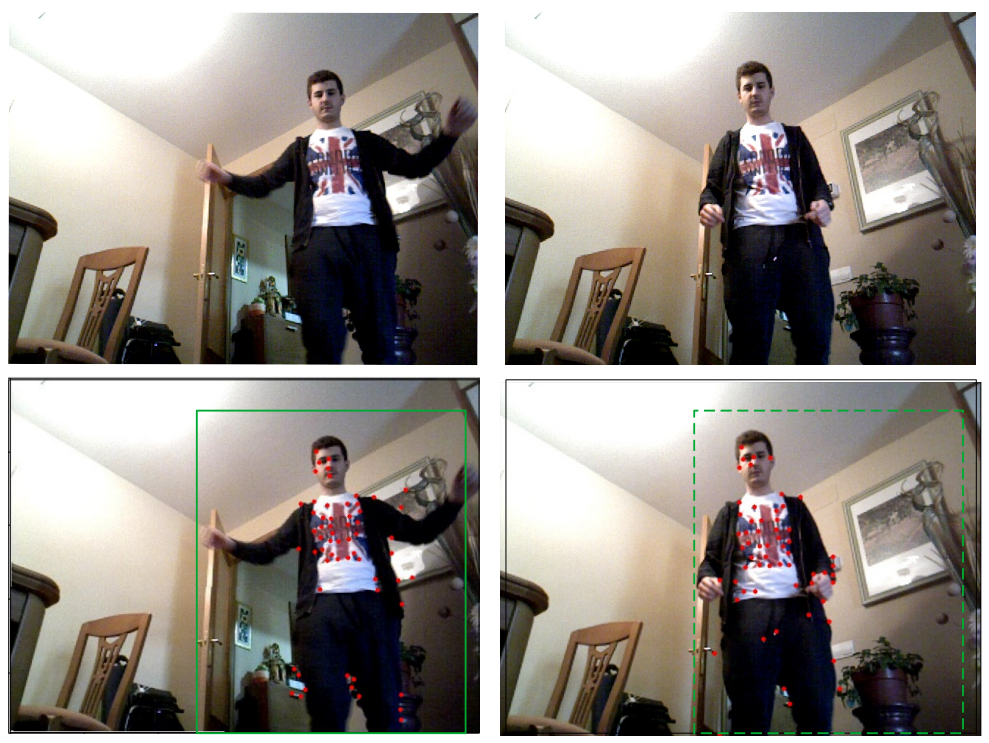
\includegraphics[width=0.9\linewidth]{tracker_demo}
	\caption{Operation of the tracking module: the last detection (green) determines the person position. The keypoints (red) are tracked during $K$ frames until the next neural update.}
	\label{fig:2_tracker_demo}
\end{figure}

As the \textit{OpenCV} implementation of Lucas-Kanade identifies the points that have been found in both frames, the average displacement of all the points can be computed. This allows to displace the bounding box of that person using the computed displacement vector. This is required, as the bounding box changes its position and size when the person moves, as \autoref{fig:2_tracker_demo} shows. Additionally, it can be rescaled in case the person moves closer or further from the camera, using the distribution of the points in the previous and current frame. As it can be seen on \autoref{fig:2_tracker_update}, the Shi-Tomasi corner detector finds a set of corners (keypoints) in the frame $t$, drawn with red points. These points are distributed with a given mean: the centroid of the cloud, represented with an "x", besides of a standard deviation pair ($\sigma_x^t, \sigma_y^t$). On the next frame, some new keypoints are found (green), whereas keypoints from the previous frame are identified. These points are useful for computing the new centroid ($\mu_x^{t+1}, \mu_y^{t+1}$) and deviations pair ($\sigma_x^{t+1}, \sigma_y^{t+1}$). With this information, the person box can be updated accordingly:

\begin{align*}
&\text{person\_coordinates}(t) = \left[\mu_x^{t}, \mu_y^{t}, w, h\right]\\
&\text{person\_coordinates}(t) = \left[\mu_x^{t+1}, \mu_y^{t+1}, w\cdot\frac{\sigma_x^{t+1}}{\sigma_x^t}, h\cdot\frac{\sigma_y^{t+1}}{\sigma_y^t}\right]\\
\end{align*}

\begin{figure}[h]
	\centering
	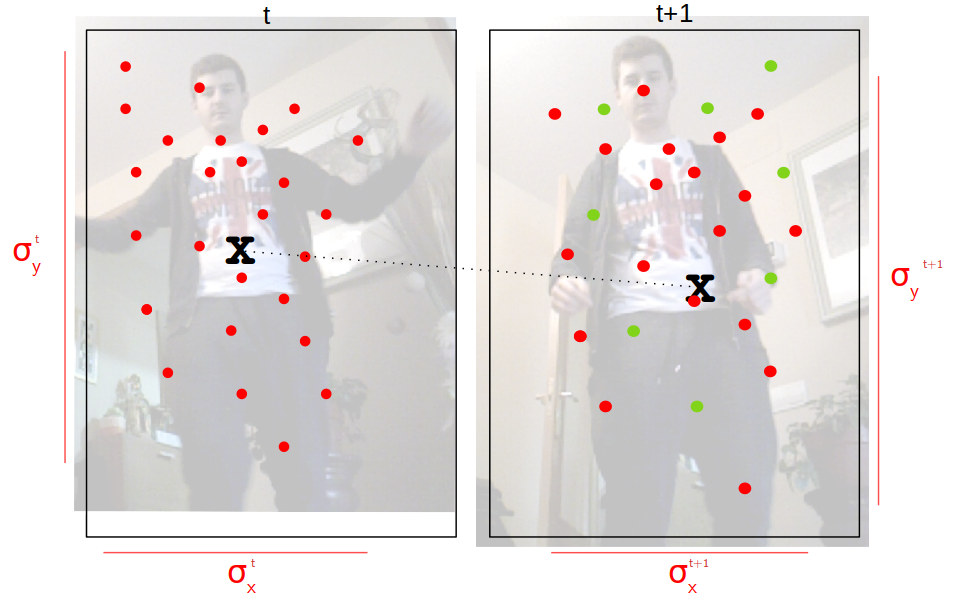
\includegraphics[width=0.9\linewidth]{tracker_update}
	\caption{Update of the Lucas-Kanade tracker from frame $t$ to frame $t+1$. The green points are the correctly detected in both frames, while red and yellow points are only detected in $t$ and $t+1$, respectively. The green points determine the new centroid and the size deformation of the box.}
	\label{fig:2_tracker_update}
\end{figure}

This way, the update is sensitive to displacements and scale changes in both directions, in case the person changes their linear distance to the camera.\\



The introduction of this Motion Tracker enhances the robustness as the output of the system will not depend just on the neural detections. This improves the performance as partial occlusions might cause some detections to be discarded momentarily. The introduction of the tracker can alleviate this effect, as the person will be kept as \textit{detected} for a number of frames even if it is not detected by the neural pipeline, and its position will be tracked using Lucas-Kanade. This number of frames is called \textit{patience}, $P$, and introduces an hysteresis in the tracker, as a person has to be lost for $P$ frames in a row to be discarded.\\



On the same way, a detection has to be maintained during $P$ frames to be joined to the tracked persons. The patience component is introduced in pursuit of stability in case the scenario complicates a stable detection. In such cases a detection flickering is observable, and this could lead to an erratic movement on the robot. The introduction of the patience solves this problem successfully.


\subsubsection{PID Controllers}
The combination of the described systems results in a efficient way to detect and identify the person to be followed, and additionally, track their movements on a fast way between slower neural detections.\\

The last block of the system is responsible of  translating this location information of the reference person into velocity commands that move the robot towards an \textit{acceptable position} with respect to the person, where certain conditions are fulfilled.\\

As it was described on \autoref{sec:2_materials}, the robot offers 2 degrees of freedom: rotation speed and linear speed. Thus, this \textit{acceptable position} can be described in those 2 dimensions:
\begin{description}
	\item[Angular position:] the reference person has to be placed at a side angle of 0º with respect to the robot front.
	\item[Linear position:] the reference person has to be placed at a distance of 1 m with respect to the robot front.
\end{description}

Due to the sensors uncertainty, the prediction and tracking estimation, and the movements of the person, these positions have to be extended to \textit{safe areas}, inside of which the robot will not trigger a velocity command for that dimension. This is achieved introducing a \textit{margin/tolerance} on each dimension. Additionally, these geometric criteria have to be translated to measurable discrepancies. This way, the safe zones can be defined as:

\begin{description}
	\item[Angular zone:] the reference person has to be placed at the horizontal center of the image, with a margin of $\pm 50$ pixels on the sides.
	\item[Linear zone:] the reference person has to be placed at a distance of 1 m with respect to the robot front, with a distance margin of $\pm 30$ cm\footnote{This criterion can be maintained in metric distance, as the depth sensor specifically yields that information. In the angular case, the image is a 2D projection on the camera plane, which does not allow to infer the relative angle with the person without extra computations using the relative distance.}.
\end{description}

These regions, which are completely tunable using the configuration file, can be visualized on \autoref{fig:2_velocity_controllers}.

\begin{figure}[h]
	\centering
	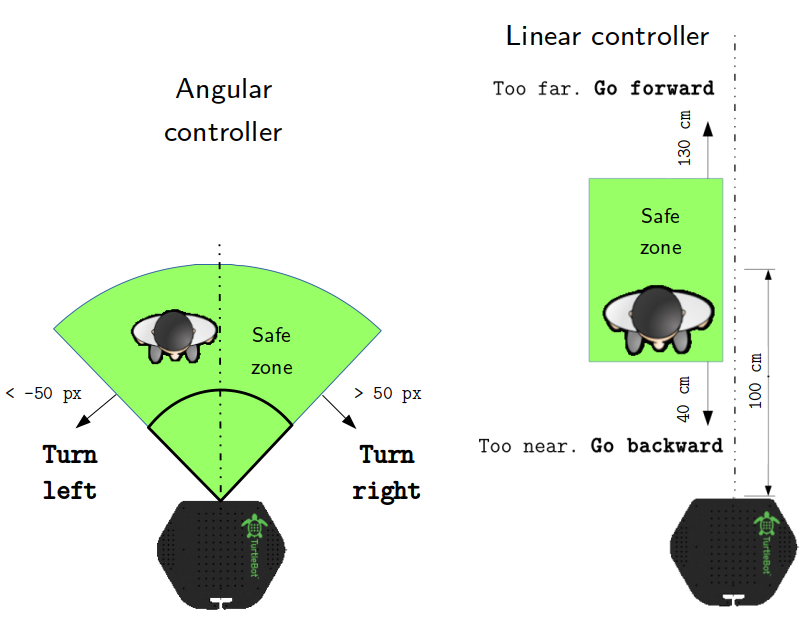
\includegraphics[width=0.7\linewidth]{velocity_controllers}
	\caption{Safe zones for each controller. Image from \cite{tfg}.}
	\label{fig:2_velocity_controllers}
\end{figure}

To place the person inside these safe zones, the robot has to move on certain directions. For determining a movement, an \textit{error} vector ($e_x, e_w$) is computed, using the tracked person coordinates:

\begin{description}
	\item[$e_x$:] the linear error or \textit{range} is computed using the depth image, estimating the distance from the robot to the person. As the Xtion sensor registers the depth image into the RGB one, the person coordinates can be used in the depth image in order to find the distance of each pixel inside the bounding box of the reference person: the \textit{person depth map}. As it is feasible that the box contains an important region of the background (specially if the person opens their arms, as the neural detection will encompass the entire body), the edges of the depth map are trimmed. Later, a 10x10 grid is computed to have 100 uniformly distributed samples of the depth of the person. In order to ensure that the background does not affect the range measurement, the median value is computed, as even if some outlier points belong to the background, they would have to make up the 50\% of the sampled set to deviate the measurement from the true range.
	
	\item[$e_w$:] the angular error can be computed taking into account that if the robot and the person are aligned, its bounding box will be horizontally placed near the center of the image. Therefore, an error metric can be extracted computing the difference on the horizontal coordinate between the image center and the center of the bounding box of the reference person.
\end{description}

These computations can be visualized on \autoref{fig:2_controller_error_computation}.


\begin{figure}[h]
	\centering
	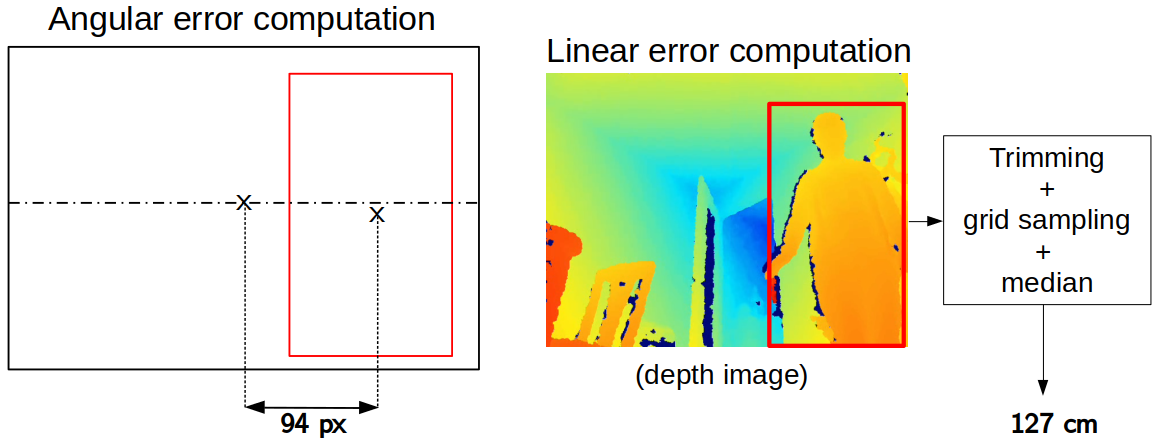
\includegraphics[width=0.95\linewidth]{controller_error_computation}
	\caption{Error computation on each controller.}
	\label{fig:2_controller_error_computation}
\end{figure}

The last step of the controller takes care of computing two proper responses (linear and angular) for the robot. If these responses depended only on the error readouts, the robot might receive unsteady commands, that might cause a total loss of the person from the field of view. This can be solved introducing a slightly more complex system: a PID controller \cite{pid_controllers}, which is a closed-loop control system that outputs a response taking into account the previously sent responses.



The \textit{PID} acronym stands for \textit{Proportional, Integral and Derivative}, as that is the methodology followed to output a response. The output in the time instant $t$, $u[t]$ depends on the currently measured error, $e[n]$, and it is computed as it can be seen on \autoref{fig:2_pid_schematic}: 

\begin{figure}
	\centering
	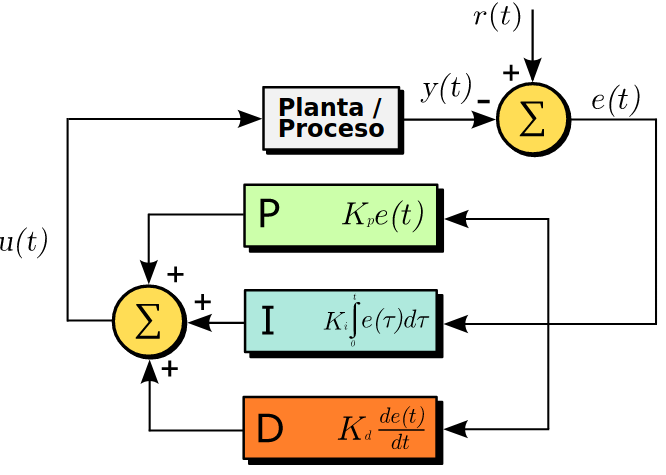
\includegraphics[width=0.75\linewidth]{pid_schematic}
	\caption{Schematic of a generic PID controller.}
	\label{fig:2_pid_schematic}
\end{figure}

This can be expressed by means of the following equation:

\begin{equation}
u[n] = k_p e[n] \ \ + \ \ k_i \sum_{i=0}^{n}e[i] \ \ + \ \ k_d (e[n] - e[n-1])
\label{eq:6_pid}
\end{equation}
This equation can be split into the three components:
\begin{description}
	\item[\textit{Proportional}:] $k_p e[n]$. This is the basic component, that computes a response directly proportional to the measured error.
	\item[\textit{Integral}:] $k_i \sum_{i=0}^{n}e[i]$. An additional response, equivalent to the sum of the total error until the current instant. This way, although a proportional response is not enough and the error gets stabilized in a non-zero value, the system will accumulate that error, increasing the response magnitude in order to close the existing gap between the error and the desired readout\footnote{When the monitored variable goes into the tolerated zone again, the total error has to be reset, as it is not required from now on.}.
	\item[\textit{Derivative}:] $k_d (e[n] - e[n-1])$. This part stands for the \emph{difference} between the last measured error and the current one, and it quantifies how well is the system responding\footnote{On systems without inertia, this contribution is generally ignored, having a simple PI control loop instead.}. If the difference is positive, that means that the system is on a further state/position with respect to the last iteration. So, in order to eliminate the \emph{inertia} the system could have acquired (which might bring oscillations and overshooting), the derivative part acts, braking or accelerating the robot depending on the value of the derivative.
\end{description}




\autoref{fig:2_pids} shows that the combination of the three sub-responses can achieve a fast and steady response (\autoref{fig:2_pids}), bringing back the system under control on an efficient way.

\begin{figure}[h]
	\centering
	\begin{subfigure}[b]{0.3\linewidth}
		\centering
		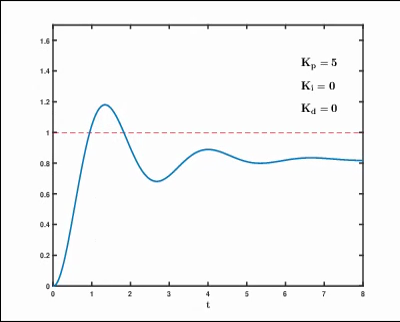
\includegraphics[width=\linewidth]{pid_p}
		\caption{Proportional.}
		\label{fig:2_pid_p}
	\end{subfigure}
	\hfill
	\begin{subfigure}[b]{0.3\linewidth}
		\centering
		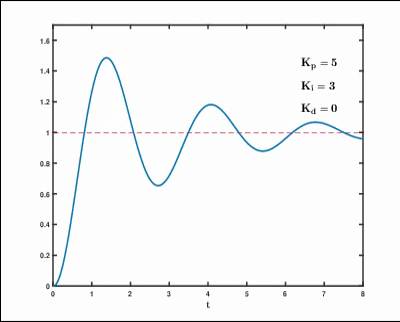
\includegraphics[width=\linewidth]{pid_pi}
		\caption{PI.}
		\label{fig:2_pid_pi}
	\end{subfigure}
	\hfill
	\begin{subfigure}[b]{0.3\linewidth}
		\centering
		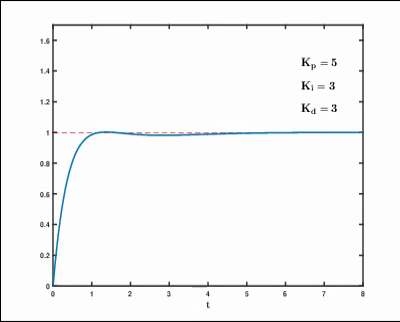
\includegraphics[width=\linewidth]{pid_pid}
		\caption{Full PID.}
		\label{fig:2_pid_pid}
	\end{subfigure}
	\caption{Different controllers response along time.}
	\label{fig:2_pids}		 	
\end{figure}

Each contribution is parameterized by its corresponding constant ($k_p, k_i, k_d$), so a task to perform is to find the optimum value for each one of them. Visual assessments of the robot stability under different combinations lead to the values present in \autoref{tab:2_pids}, which yielded a steady behavior of the robot when it is subject to typical indoor conditions of following a wandering person. As for previous parameters, all these values can be changed using the configuration file.

\begin{table}[h]
	\centering
	\begin{tabular}{|c|c|c|}
		\hline
		\textbf{} & \textbf{Linear} & \textbf{Angular} \\ \hline
		$k_p$     & 0.4               & 0.005               \\ \hline
		$k_d$     & 0.04              & 0.0003              \\ \hline
		$k_i$     & 0.05              & 0.006               \\ \hline
	\end{tabular}
	\caption{Optimal found values for the parameters in each PID controller.}
	\label{tab:2_pids}
\end{table}

Finally, when the speed is computed, it is adapted to a ROS \texttt{Twist} message, and it is published to the topic devoted to velocity commands to the robot. On the other side of the topic, the driver reads these messages and moves the robot accordingly with the commands received.\\

This last block completes the design of the full proposed person following behavior.

\section{Software architecture}

The developed software puts all the previous components together, offering two application modes:
\begin{description}
	\item[\texttt{followperson} mode:] this is the default mode of the system. When running on this mode, the program feeds the tracker and the neural pipeline with images from the ASUS Xtion, and sends the velocity commands to the robot, writing them into the specified ROS topic.
	
	\item[\texttt{benchmark} mode:] this mode is designed to test the entire infrastructure, with the purpose of tuning parameters or extracting objective metrics for comparisons, such as precision, or inference time. The images are read from a previously recorded ROSBag, emulating the Xtion sensor and providing always the same RGBD sequence to be fed in different implementations, allowing to compare the performance of different configurations under identical conditions. On this mode, the velocity commands are not sent to the robot, just drawn in the output image (\autoref{fig:2_output_image}), which is also saved into an output video for later visualization. Aside of the video, execution graphs and YAML\footnote{YAML is a plain-text data serialization format. It has been chosen as a standard format on this project as it offers a good tradeoff between serialization (allowing the data to be converted back into data structures in Python) and  readability of the file without processing it.} files are stored containing information about the tracked persons and times for each frame processed by the \texttt{Main} thread.
\end{description}

This mode, and other parameters, can be configured on the program execution without modifying the source code. The program receives a YAML configuration file specifying all the required parameters in order to run the system:

\begin{lstlisting}
NodeName: "followperson"
Benchmark: true # true for benchmark, false for followperson
RosbagFile: "resources/bag1.bag"  # path to the ROSBag if benchmark 
LogDir: "resources/benchmarks" # where to write the results

Networks:
  # Parameters for the neural pipeline
  Arch: ssd # detection architecture [ssd, yolov3, yolov3tiny]
  DetectionModel: "models/ssd_mobilenet_v1_0.75_depth_coco.pb"
  DetectionWidth: 416 # usually 300 for SSD, 416 for YOLOv3tiny
  DetectionHeight: 416 # usually 300 for SSD, 416 for YOLOv3tiny
  FaceEncoderModel: "models/facenet_inception_resnet_vggface2.pb"

RefFace: "resources/ref_face.jpg" # Image of the reference face

Topics:
  RGB: "/camera/rgb/image_raw" # topic publishing the RGB images
  Depth: "/camera/depth_registered/image_raw" # topic publishing the depth images

# Parameters for the speed controllers
XController:
  Kp: 0.4
  Ki: 0.04
  Kd: 0.05
  Min: 0.7
  Max: 1

WController:
  Kp: 0.005
  Ki: 0.0003
  Kd: 0.006
  Min: -50
  Max: 50
# Parameters for the people tracker
PeopleTracker:
  Patience: 5
  RefSimThr: 1.0
  SamePersonThr: 60
\end{lstlisting}


The previously depicted structure can be implemented on the Jetson board using the programming language Python. As the tracking module has to run asynchronously, the \texttt{threading} library is used, deploying the following threads:

\begin{description}
	\item[Main thread:] the purpose of this thread is to continuously draw the output image (shown in \autoref{fig:2_output_image} and explained below), and compute the errors and suitable responses, as well as sending them to the robot. One thing to notice about this thread is that it does not process all the frames in the sequence, as its rate depends on the drawing time and the computation time of the response. It works asynchronously, fetching the latest frame from the \texttt{tracker} thread.
	
	\item[\texttt{networks\_controller} thread:] this controller handles the 3 described neural networks, running sequential inferences on them. In the Jetson platform, these neural networks are deployed in the GPU of the board. Therefore, this thread can be seen as the one which interacts with the GPU in order to pass, retrieve and transform tensors from the networks.
	
	\item[\texttt{tracker} thread:] as it was shown before, the tracker must inherently iterate at a higher rate than the neural infrastructure. However, including it in the main thread would be bad for its performance, as the speed would be limited by the image drawing and responses publication in the speed topics. Therefore, it is extracted to an specific thread. The simplicity of the Lucas-Kanade tracker makes it fast to execute, however it would be pointless to track a person several times before a new image arrives from the camera. To avoid this, the thread has a rate limitation of 30 Hz, equal to the framerate of the Xtion sensor.\\
	
	As this is the fastest thread to execute, and it is crucial that the tracker has access to each and every image from the camera, this is the first component to receive the images from the source, on a 30 Hz synchronous manner. The rest of components can fetch the images asynchronously from the tracker whenever they need them.
	
	\item[ROSCam:] this component, responsible of fetching the images from the source (a ROSBag or the Xtion camera, as explained before), is not deployed as a thread. However, as it works by means of subscribers when a synchronous mode is required (thus, when the source is the Xtion camera), the ROS API for Python, \texttt{rospy} automatically deploys these subscribers on independent threads.
\end{description}

This software architecture can be seen in \autoref{fig:2_software_architecture}, where the interaction between the threads can be visualized. The \texttt{Main} thread varies its behavior depending on the configured mode (\texttt{followperson}/\texttt{benchmark}), whereas the rest of threads  behave similarly in both configurations.

\begin{figure}[h]
	\centering
	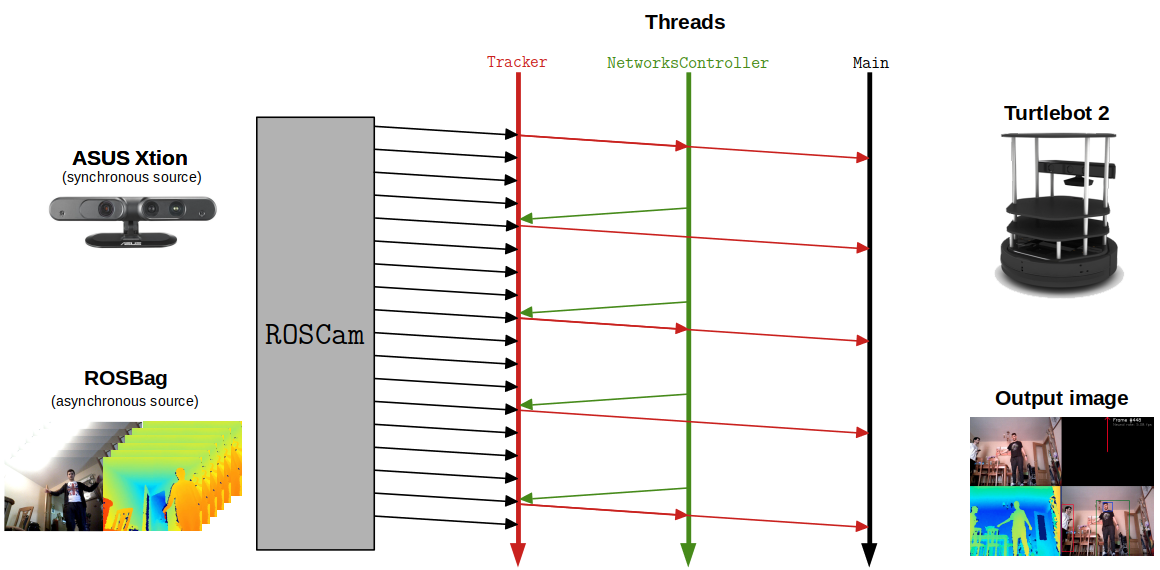
\includegraphics[width=0.8\linewidth]{software_architecture}
	\caption{Software architecture for the system.}
	\label{fig:2_software_architecture}
\end{figure}



The visible output of the system is the image shown in \autoref{fig:2_output_image}. This image is drawn by the main thread, when the position errors are computed and the responses have been sent to the robot, and it serves for monitoring the execution, showing the images, the tracked persons and the sent commands. If the benchmark mode is enabled, these image are appended to a output video, which serves for posterior visualizations or assessments of the performance.

\begin{figure}[h]
	\centering
	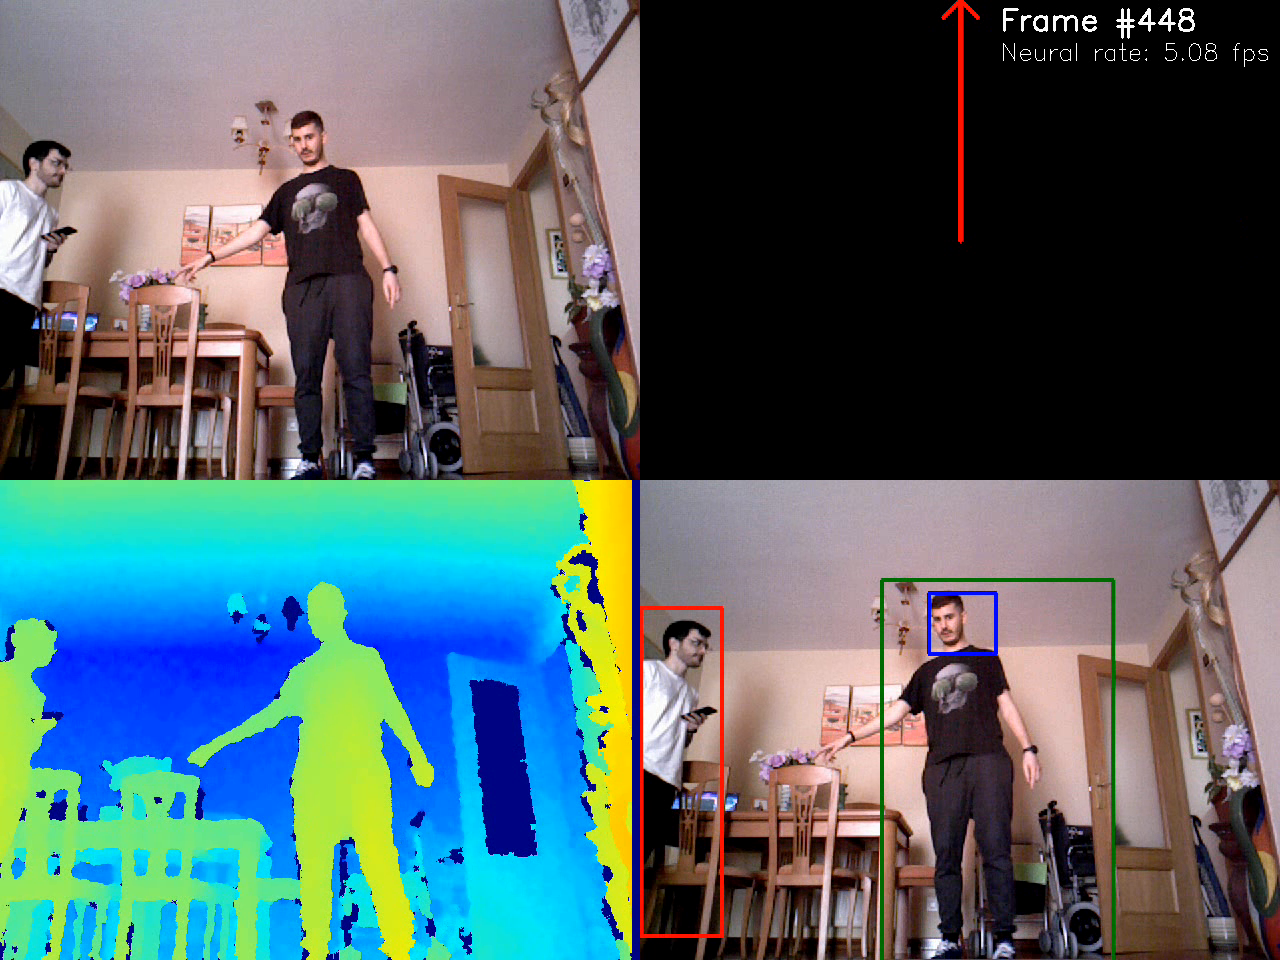
\includegraphics[width=0.85\linewidth]{output_image}
	\caption{Output image drawn by the program. Upper left: input RGB image. Bottom left: input depth image. Upper right: velocity commands sent to the robot, and information about the neural rate and number of current frame. Bottom right: tracked persons (green if it is reference, red otherwise) and their faces}
	\label{fig:2_output_image}
\end{figure}




